% wfbook
% wfbook.tex

\documentclass[12pt,UTF8]{ctexbook}

% 设置纸张信息。
\usepackage[a4paper,twoside]{geometry}
\geometry{
	left=25mm,
	right=25mm,
	bottom=25.4mm,
	bindingoffset=10mm
}

% 图片相关设置。
\usepackage{graphicx}
\graphicspath{{Images/}}

% 设置字体,并解决显示难检字问题。
\xeCJKsetup{AutoFallBack=true}
\setCJKmainfont{SimSun}[BoldFont=SimHei, ItalicFont=KaiTi, FallBack=SimSun-ExtB]

% 目录 chapter 级别加点(.)。
\usepackage{titletoc}
\titlecontents{chapter}[0pt]{\vspace{3mm}\bf\addvspace{2pt}\filright}{\contentspush{\thecontentslabel\hspace{0.8em}}}{}{\titlerule*[8pt]{.}\contentspage}

% 设置 part 和 chapter 标题格式。
\ctexset{
	part/name= {第,卷},
	part/number={\chinese{part}},
	chapter/name={第,篇},
	chapter/number={\chinese{chapter}}
}

% 设置署名格式。
\newenvironment{shuming}{\hfill\bfseries\zihao{4}}

% 注脚每页重新编号,避免编号过大。
\usepackage[perpage]{footmisc}

\title{\heiti\zihao{0} wfbook}
\author{WangFei}
\date{\today}

\begin{document}

\maketitle
\tableofcontents

\frontmatter

\chapter{前言}



\mainmatter

\chapter{生殖器官}

\section{女性生殖器官}

女性的生殖器官包括外生殖器官和内生殖器官两部分。外生殖器主要是指阴阜、大阴唇、小阴唇、阴蒂、阴道前庭、尿道口、阴道口、处女膜、前庭大腺和前庭球,而内生殖器则包括阴道、子宫、输卵管和卵巢。

\subsection{外生殖器官}

阴阜在耻骨联合前方,由皮肤及很厚的皮下脂肪层构成。到性成熟期常有阴毛,分布呈倒三角形。

外阴靠近两股内侧的一对长圆形隆起的皱襞为大阴唇。大阴唇外面长有阴毛,皮下是脂肪组织、弹性纤维及静脉丛。生育前大阴唇自然合拢,生育后向阴阜两侧分开。大阴唇内侧有一对小阴唇,是一对黏膜皱襞,表面湿润,有丰富的神经分布,因而感觉敏锐。

阴蒂位于两侧小阴唇之间的顶端,是一个长圆形的小器官,末端为一个圆头,内端与一束薄薄的勃起组织相连接。勃起组织有丰富的静脉丛和神经末梢,是女性最重要的性感区,对其进行爱抚会引起强烈的性反应。

两侧小阴唇之间的凹陷部分是阴道前庭,阴道前庭表面有黏膜遮盖,前半部有尿道开口,后半部有阴道开口。尿道口是一个形状不規则的橢圆小孔,尿液从这里流出。

阴道口被一塊不完全封閉的黏膜所遮盖,中间是处女膜。处女膜的正反两面都是湿润的黏膜,黏膜之间有结缔组织、微血管和神经末梢,中间的小孔即处女膜孔,经血即由此流出。处女膜孔的大小和膜的厚薄程度因人而异。处女膜破后,黏膜变成许多小圆球状物,成为处女膜痕。

阴道口的两侧有前庭大腺(又称“巴氏腺”),能分泌液体,有滑润功能。前庭大腺有小蚕豆般大小,性兴奋时能分泌黄白色黏液,起滑润阴道口作用。正常检查时摸不到此腺体,如有感染时则会肿大。前庭球又称为“球海绵体”,是一对海绵体组织,位于阴道口两侧,能勃起。

\begin{figure}[htbp]
	\centering
	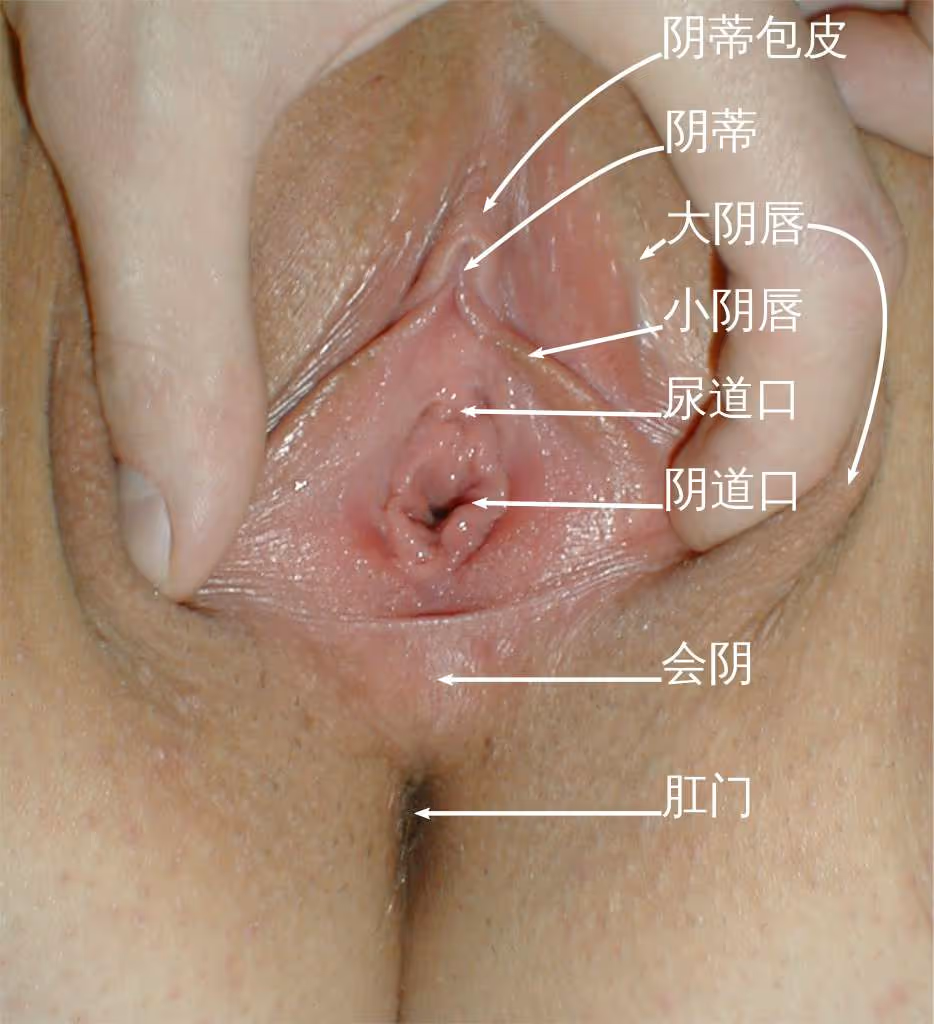
\includegraphics[width=0.7\linewidth]{1}
	\caption{}
	\label{fig:1}
\end{figure}

\begin{figure}[htbp]
	\centering
	
\includegraphics[width=0.7\linewidth]{2}
	\caption{}
	\label{fig:1}
\end{figure}

\subsection{内生殖器官}

卵巢呈卵圆形,位于盆腔内子宫的两侧,左右各一。卵巢发育成熟后,能产生成熟的卵子,并分泌雌性激素,维持女性特征。在一个月经周期中,卵巢内常有几个甚至十几个卵泡同时发育,但一般只有一个发育成卵子。

输卵管位于子宫两侧,是输送卵子进入子宫的弯曲管道。输卵管内端与子宫腔相通,外端游离。输卵管管壁由黏膜、肌层及外膜三层组成。黏膜上皮为单层柱状纤毛上皮。纤毛具有摆动功能。肌层的蠕动及纤毛的摆动,有助于受精卵进入子宫腔内。

子宫位于骨盆腔内,在膀胱与直肠之间,形状似倒置的梨子,前后略扁,分宫底、宫体、宫颈三部分,上通输卵管,下接阴道。

子宫是孕育胎儿的器官,又是产生月经的场所。子宫壁共分三层,由外向内为外膜、肌层和内膜。

阴道是一种收缩性很强的肌性管道,上通子宫颈管,下开口于阴道前庭,阴道前壁紧贴膀胱和尿道,后壁与直肠相邻。阴道为性交器官,又是月经排出和胎儿娩出的通道。

\begin{figure}[htbp]
	\centering
	
\includegraphics[width=0.7\linewidth]{3}
	\caption{}
\end{figure}

\section{男性生殖器官}

男性生殖器官分为外生殖器官和内生殖器官两部分。外生殖器包括阴阜、阴囊和阴茎,而内生殖器由睾丸、附睾、精索、输精管及射精管、精囊腺、前列腺、尿道球腺、尿道等组成。

\begin{figure}[htbp]
	\centering
	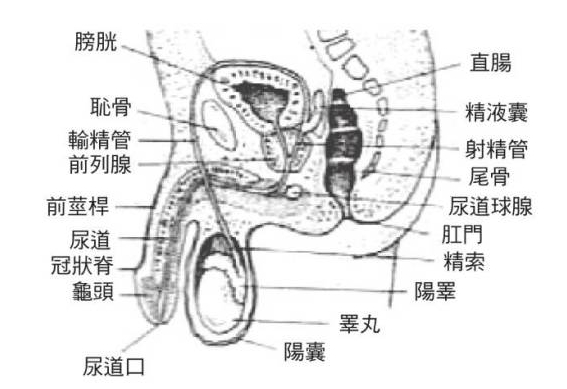
\includegraphics[width=0.7\linewidth]{4}
	\caption{}
\end{figure}

\subsection{外生殖器官}

阴阜为耻骨前方的皮肤和丰富的皮下脂肪组织。青壮年时阴阜显著隆起,中年以后脂肪组织减少下陷,老年则萎缩变平。

阴囊是由皮肤、肌肉等构成的柔软而富有弹性的袋状囊,里面有睾丸、附睾、精索,主要功能有保护睾丸、调节温度、有利于精子的产生和贮存等。阴囊内有阴囊隔,将阴囊内腔分成左右两部分,各容纳一个睾丸和附睾。阴囊皮肤薄而柔软,并有很多的褶皱。阴囊皮肤有明显的色素沉著,长有稀疏的阴毛。

阴茎后部为阴茎根,中部为呈圆柱形的阴茎体,其前端膨大部分为阴茎头(俗称“龟头”)。阴茎轴与阴茎头之间是冠状沟,阴茎头与冠状沟含有丰富的神经末梢,对刺激是很敏感的,而冠状沟处神经分布最丰富,敏感性最高。阴茎体由阴茎海绵体和尿道海绵体组成,具有丰富的血管、神经、淋巴管。从外形上看,阴茎有松弛和勃起两种状态,具有排尿、性交、射精三大功能。

\subsection{内生殖器官}

睾丸是男性生殖腺,呈卵圆形,左右各一,由精索将其悬吊于阴囊内,长约4~5公分,厚约3~4公分,约重15公克左右。睾丸是产生雄性生殖细胞(即精子)的器官,也是产生雄性激素的主要内分泌腺体。

附睾位于睾丸的后外侧,外形细长,似半月形,左右各一,长约5公分。附睾有储存和排放精子、促使精子成熟及供给精子营养的作用。

精索位于睾丸上端至腹股沟管腹环之间,左右各一,全长约14公分。精索是睾丸、附睾及输精管血液、淋巴液循环的通路,也是保证睾丸的生精功能及成熟精子输送的主要途径。输精管是精索内的主要结构之一,其末端与精囊腺的排泄管汇合成射精管,穿过前列腺,开口于尿道,全长约40~46公分,直径约2~3公厘。

输精管是精子从附睾被输送到前列腺部尿道的唯一通路。射精管是输精管壶腹与精囊管汇合之后的延续。射精管很短,长仅为2公分左右,管壁很薄。

精囊腺为一对扁平长囊状腺体,左右各一,表面凹凸不平呈结节状,其末端细小为精囊腺的排泄管,与输精管的末端汇合成射精管,在尿道前列腺部开口于尿道。精囊长4~5公分,宽约2公分,容积约4C.C。精囊为屈曲状的腺囊,其分泌液主要为精浆液,占精液的70\%左右,对精子的存活有重要作用。

前列腺为一个栗子状的腺体,平均重量约20公克,是男性最大的附属腺体,能分泌前列腺液,组成精浆液。前列腺还被认为是一个性敏感部位,对其进行适当刺激时,可以引起性兴奋。

尿道球腺左右各一,位于尿道生殖隔上下筋膜之间的会阴深囊内,开口于球部尿道近端,可分泌少量液体,为精浆的成分之一。

男性尿道长12~20公分,既有排尿功能,又有排精的功能。

其中有尿道球腺,可分泌液体,参与精液的组成,性交时有润滑阴茎头的作用。

\chapter{性欲}

简单地说,性欲就是对性生活的一种欲望,它既受体内激素水准的调节,也受社会、家庭等周围环境因素的影响。同时存在比较大的个体差异,即使是同一个人,性欲的高低也随年龄、心理状态、患病状况、生活品质、工作环境、婚姻状态等不同而表现不同。

一般情况下,性欲源于性心理的驱动,比如对异性的爱慕可以诱发性欲。男女之间建立美满家庭以及夫妻间的亲昵,都会产生性交的欲望。性欲产生的另外一个原因与内分泌有关。青春期过后,骤然提高的人体性激素分泌水准会驱动性欲。男性精囊、前列腺等性腺内分泌物的增加与淤积,女子外阴前庭大腺等分泌物的过多贮存,都可诱发性刺激和促进性欲。此外,既往性生活的愉快感受,或者男女之间身体接触产生的性刺激等,也可以诱发性欲。所以,性欲是多方面因素综合作用的结果,不但思维、意识、情感、环境等因素与性欲相关,而且语言、文字、图书、音乐等,也会给性欲带來举足轻重的影响。

\section{男人的性欲和女人的性欲一样吗?}

从表面上看,男人的性欲似乎比女人强,因为在性生活中居于主动地位的女性比较少,这里面既有生理上的因素,但主要还是心理因素的影响。许多女人习惯于压抑自己的性需求,所以,在多数情况下,男人的性欲表现得比女性主动,但这不证明男人的性欲就比女人的性欲强。

处于青春期的男性比女人更富于性幻想,并容易将感情需要和性需要混为一谈。成年以后,工作的压力和家庭的负担,会使青春期旺盛的性渴望减弱,但仍有少数人性欲一直比较强烈,在这一点上,女人和男人是一样的。男性的性欲在某些年龄阶段表现得要比女人强,但在另一些年龄阶段却可能完全相反。在性生活不和谐的夫妻中,产生性欲低下的一方往往是丈夫,其中年龄是个重要因素,男人的性欲高潮期通常在30岁以前,而女人则是在40岁左右,才对性活动表现出浓厚的兴趣。
===========================================
\section{为什麼有的人性欲强,有的人性欲弱}

性欲是有很大的个体差异的。性欲的强弱程度与下列因素有关:

①遺傳因素:性欲的强弱程度受遺傳因素的影响,一个家族的成員,往往表现出類似的性欲傾向。

②激素水准:人体中有多种激素,男女皆然。在多种激素中,雄性激素对性欲的影响最大。雄性激素水准高,性欲就强,雄性激素水准低,性欲就弱,無論男女都一样。

③感觉刺激:在多种刺激下,人体就会产生各种各样的感觉,如視觉、味觉、聽觉、嗅觉、触觉等,这些感觉可以激起性欲,在这一点上男性和女性沒有明显差异。

④性体驗和性经驗:如果以往性体驗順利并且性经驗丰富,性喚起就比较容易;反之,性欲的产生就比较困難。

⑤环境因素:人体会对外界环境的刺激作出多种反应,所以生活环境中的光照、温度、濕度、季节、飲食等因素,都会影响性欲的产生。

⑥文化因素:性欲的产生是一种个人行为,但性欲也与文化因素有关,在某种程度上它必須接受倫理、法律、道德,甚至醫學的约束。

⑦情緒变化:心理状态影响著性欲的产生,比如當人們被憂慮、恐懼、憤怒、抑鬱、疼痛、痛苦所困擾的时候,一般是很難产生性欲的。

⑧年龄因素:人的性欲会随著年龄的变化而变化。就一般規律而言,男性的性欲高峰在30岁之前,而女性则是在40岁以后性欲最为高漲。随著年龄的增加、内分泌的改变,体内雄性激素的减少,人体感觉会变得遲鈍,導致性器官血液循环不良,再加上來自事業、生活及社会交往等方面的压力,这些因素都会使人的性欲减退。

⑨健康因素:健康的生理状态是维持性欲的基礎。人体的各种疾病,如内分泌、生殖器官、代謝系統、肿瘤及其他消耗性疾病,都会影响性欲的产生。

總之,性欲是人的生理本能之一,它受多种因素的影响。

\section{不要将性欲望和性功能混为一谈}

现實生活中,不少人对性都存在认识上的誤区,将性欲望和性功能混为一谈即是其中之一。實際上,这两者还是有区別的。

所謂性欲望是对性的一种要求、一种渴望的心情,而性功能则是将欲望化做具体行为的能力,完美和谐的性生活,需要性欲望和性功能的協调和統一。如果能将性欲望和性功能協调于一身,就能充分享受性所带给自己的愉悅;但是要想實现这个願望,需要不斷地摸索和探尋,如果沒有完成这种轉化,就会導致性的各种不和谐和性功能障礙。

實際上,性欲望和性功能分离的情况是很常見的,常見原因有生理性的,也有精神心理性的,还有疾病等因素。比如,进入青春期的青少年,开始出现朦朧的性意识,也具有了阴茎勃起的能力,但他們对性的欲望还沒有建立起一个明確的概念;一个习惯自慰的青年,有可能擔心自己患了陽痿,懷疑自己的性能力;老年男性,儘管岁月的磨煉使他們更加珍爱生活、珍爱爱情,对于性的要求(欲望)也很高,但是性功能却在慢慢地减退,直至消失;患有某些疾病的男子,儘管主觀上很想「要」,但實際能力却不行;某些傳染病患者,儘管性功能很好,但为了疾病的康復,必須抑制自己的性欲望。

\section{性生活不仅仅意味著性交}

性生活是夫妻间表達感情、傳遞爱意的重要手段。在正常的夫妻性生活中,即使男性最終出现了高潮和射精,但这也并不是性生活的全部内容,更不是它的首要目的,性生活还包括夫妻雙方的精神交流、性生活中的默契配合和性交后的恩爱,性生活的品质,在很大程度上,取決于全部过程的圆满程度。

有些人常把性交过程看做是第一位的,于是導致了性生活的过于急切、粗暴和简单的程式化。丈夫容易忽視妻子的情感需求,把性生活简化成一系列的动作,甚至有人为了显示自己“性能力强”,而粗暴地强迫妻子与自己过性生活,極大地傷害了妻子的人格与情感。这种「性」多、爱少的方式,只会给对方带來痛苦和厭惡,而不是身心愉悅。其實多数女性最看重的并不是性交的过程,而是相互温存的感觉与感情交流。

有关调查显示,夫妻中大约有四分之一的人几乎从不相互親吻;差不多有一半的男性很少抚摸妻子,但他們均认为自己的婚姻生活是和谐美满的,或者是比较满意的。由此可見,多数男人往往是过分地偏爱最終的性交过程,这种现象在鄉下更为普遍,有些人只是把性看作是一种生活内容,是必須履行的義務,而不是为了傳遞爱。

现實生活中,家庭、職场有很多問題都要面对,身心疲憊的情况会时有发生。如果夫妻中的一方想要过性生活,而另一方则状态不好只是勉强为之,那麼性生活结束之后,不仅主动的一方会觉得毫無兴致,而被动的一方也会更加難过甚至痛苦,長期下去会形成惡性循环。事實上,越是突发地匆匆行事,就越是極其狹隘地理解性生活的内容,也就越缺乏交流和深切感受,身心疲勞也就越是加重,结果把性生活变成消極、冷漠和缺乏激情的「機械化運动」,夫妻雙方難以体会性生活带來的愉悅感,甚至出现性功能障礙和性冷淡,并由此喪失了爱心、情趣及性的和谐之美。过去这种情况在中年男人身上比较多見,但近些年一些年轻人,甚至新婚不久的男性也抱怨「沒意思」,其實是同样的原因所導致。因此,無論男人还是女人都应該切記:为了爱而性交,而不是为了性交而性交。把握好这个基本点,一切的問題也就順理成章地容易解決了。

\section{性交时应適时插入}

性交是夫妻生活的重要内容,关係到夫妻感情的和谐与否,所以夫妻雙方不应草率从事或敷衍应付,在性交前要做好充分的准備工作。在性刺激下,男女雙方的性器官都会逐步处于充血状态,男性阴茎膨大了,女性阴道也有变化,但这些变化所需的时间,男女有很大的差异。當男性的性欲達到一定的程度,阴茎勃起变硬时,多数男人著急要进入下一步工作,但女方性欲的激发,往往需要一定的时间,短的需要几分鐘,長的可在半小时以上。當然,有性交经驗以后,夫妻之间的差异会缩短,并基本保持一致。

性交时男女雙方的体内,都会分泌出具有润滑作用的液体,有助于激发性兴奋。此时男性阴茎上端的阴茎头被润滑的液体所滋润,女性阴道外及阴道内壁也都分泌著这种物质,男性阴茎靠著这些润滑的液体,插入女性阴道会变得容易,但是如果男性性急,在这种润滑的液体分泌之前,便要插入女性的阴道,再加上动作粗暴,不但容易使女性受傷,也会使女性产生恐懼性交的心理,还会给自己的性器官带來明显不適(疼痛甚至損傷),给以后的性生活造成障礙。所以在性交前做充分的准備工作是非常重要的。

\section{怎样理解性快感}

性快感是性生活中的一种心理感受,雖然目前还沒有具体的量化指標,但界定它的程度,可以从以下几个方面去体驗它的存在。

首先是宣洩后的轻松感。男性在性刺激下产生性兴奋,阴茎勃起,产生交媾的欲望,達到射精。射精之后恢復平静,心境弛緩,獲得宣洩后的满足,这是性快感的内容之一。

其次是夫妻情感的交汇融合。夫妻恩爱,相互温存相偎,进行爱抚,引发性衝动而进入性高潮。性高潮之后,雙方进一步温存、体贴,会产生一种发自内心的愉快。

性快感的另一内容是在疲勞中体会快乐。从性兴奋的产生到最后射精结束,雙方都有高强度付出后的疲勞感,这种疲勞感其實也是一种無聲的交流,其产生的快乐是其他事情難以取代的。

總而言之,性快感不仅仅是性器官的感觉,必須从情感、心理和行为中去感受它的存在。单純的性宣洩是粗野的行为,是不可能产生完美快乐的感觉的。

\section{性生活的几个阶段}

性生活大体有四部分的内容,即性交的預備、性器的交合、性行为的運动、性交的结束。这个过程又可以分为兴奋期、平臺期、高潮期和消退期。

①兴奋期:在肉体或精神上的性刺激下,性欲被喚起,身体开始处于紧張阶段。

②平臺期:即性高潮前期,在这个阶段的基礎上,身体的性紧張逐漸到達顶峰。

③高潮期:持续时间很短,大约只有几秒鐘的时间,高度紧張的肌肉经过痙攣,处于放松的状态,使人獲得快感。

④消退期:身体由紧張逐步松弛和消散的过程。

性生活的不同阶段,男女雙方的身体都会出现相应的生理变化,但是这种变化是存在很大的个体差异的。

\section{射精和精液的主要成分}

男性在性高潮或遺精时,精液通过输精管、精囊、射精管、精阜开口及尿道被排出体外,这便是射精。

\begin{figure}[htbp]
	\centering
	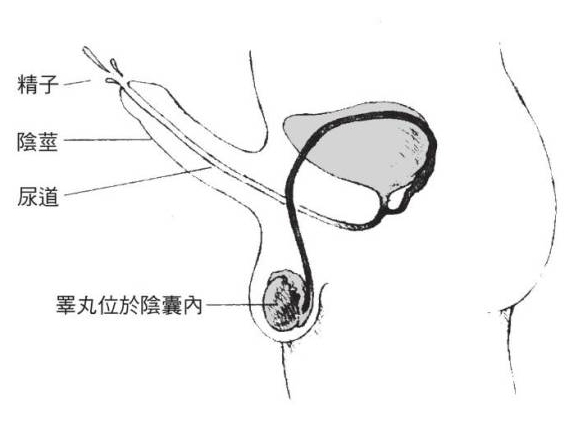
\includegraphics[width=0.7\linewidth]{5}
	\caption{}
\end{figure}

一般情况下,一位男性每次排出的精液为2~6C.C,每C.C含成活的精子为6千万~1.5亿个左右。精液是由精子和精浆组成,精浆又包括前列腺液、精囊液和尿道球腺液等成分,其中前列腺液约占三分之一,精囊液约占三分之二。精浆負責输送精子,并为精子提供能量和营养物质。精浆中主要成分是水,此外还有糖類、電解质、酶類、维生素等物质,这些营养物质是保证精子生存与活动的物质基礎。各种液体射出的先后順序为:首先射出的是约0.1~0.2 C.C的尿道球腺液,接著射出的是總量约0.5C.C的前列腺液和精子,最后射出的是约2.0~2.5C.C的精囊液。

\section{男性怎样判斷自己的性功能}

性功能是人類的基本本能之一,在生活中的地位是不容忽視的。健康、完善的性功能,不仅是身体健康的標誌,而且还影响著人的精神状态、生活品质、生育后代的能力,以及人格魅力等方面,同时也是性文化中不可缺少的一部分。

怎样判斷自己的性功能、如何对待自己的性功能,如果缺乏必要的知识积累,難免会走入誤区。比如,有的人一旦发现自己的性能力出现一些变化就憂心忡忡,陷入焦慮和困惑,懷疑自己是不是性功能减退了,終日疑神疑鬼,亂吃補藥,或者偷偷地去找江湖庸醫,结果問題不但沒有解決,还引发了別的麻煩。事實上,相當一部分懷疑自己性功能有問題而前去就醫的「患者」,在经过相关的醫學检查后,并沒有发现有什麼疾病,所謂的性功能减退,實際是过度紧張造成的。

还有一些人与上述这些人不同,他們一旦发现自己的性功能有問題,「死要面子活受罪」,遲遲不肯看醫生,長期生活在巨大的精神压力下,當情况发展到非常嚴重的地步、不得不就醫时,往往病情已经很嚴重,治療起來自然相當困難。

怎样正確評價自己的性功能呢?以下几点供参考:

(1)关注性器官的勃起状态

年轻且身体健康、精力旺盛的人無論何时,一旦有性方面的刺激,都会对性产生兴趣,阴茎能迅速勃起;年紀稍長一些的中年人,可能会在勃起之前需要一段时间,这些都是正常的。但如果你发现自己的性器官有时候勃起,有时候不能勃起,或者雖能勃起,但堅持不了多長时间,未到射精时就疲软下來,这种情况常常提示你的性功能可能有所降低,但問題不大,可以通过适当的食補、正確的藥補,及科學的鍛鍊进行糾正。比较嚴重的情况,是在较長的一段时间里,阴茎始終沒有勃起过,这就需要看醫生了,应該到醫生那裹接受检查后,再採取相应的措施。

(2)判斷自己性欲产生的方式

性欲比较旺盛的人,一般都会在性生活中处于主动地位。在有些两性关係中,如果男女雙方的性欲强度差不多,常常是男女互为主动,當然也不排除女方主动的情况。如果女方主动,男方能夠积極回应,就大可不必为自己的性功能擔心。如果你在性生活中表现得很消極,必須依賴对方的主动,或者即使对方主动诱導,也很難激起你对性的兴趣來,说明你的性能力出现了問題。

性能力出现問題,不要消極迥避,积極的应对措施是尋求專業醫生的幫助。除了男科醫生外,諮詢心理醫生也是十分必要的。如果沒有器质性疾病,措施得當,問題并不難解決。只是一定要科學就醫,而不是消極迴避或「有病亂投醫」。

3)对性的关心程度是性功能的一种表现

性功能包括性生理和性心理两方面的内容。一般情况下,性心理和性生理正常的男性,無論年龄多大,一旦看見性感、年轻、漂亮的女子,都会情有所动,看見妻子裸露的肌肤,「肤色如凝脂」,就会有想抚摸的衝动,这是正常的性反应,不能一概歸结为「下流」。如果遇到和自己关係很親近、很鍾情的女性,只能产生一般的交谈所带來的快乐,而不产生任何性的想像,说明你的性感受开始变得遲鈍了,需要想辦法去提高自己的性兴奋程度,像治療軀体的其他疾病那样,尋找病因,进行对症治療。

\section{適时变换性交姿勢}

经过磨合之后,夫妻性生活时的姿勢往往就固定下來了,久而久之,可能一如當初时那样美满,但也可能由于一成不变的固定模式,導致性生活品质下降。正確的做法是偶有变化,雖然并不一定嘗試每种姿勢。

性交姿勢又叫性交体位,对性反应的性质和强度,都有很大的影响,如果性交体位不適宜,就会造成性兴奋程度的下降。沒有哪一种体位適合于所有的配偶,因此要对其进行探討。夫婦雙方的性器官未必十分吻合、贴切,有大、小方面的不適应,要根據这种不適应用不同的体位來補救,并找出最容易達到性高潮的体位。由于性交体位的改变,有助于提高性生活的品质,所以夫妻雙方要密切配合,找出更理想、更適合于自己身体條件,和更有利于性感满足的新姿勢來,比如可以在一次性交过程中,由一种体位变換到另一种体位,甚至变換好几种体位。常用的性交体位有如下几种:

(1)男上女下(女仰臥、男俯)

这是最傳統、最常用的性交体位。随著歷史和性文化的发展,人們的人文理念、文化修養、社会习俗,都早已发生了深刻的变化,「男上女下」已不是唯一「正統」的性交体位,人們勇敢地进行著新的嘗試,但「男上女下」的体位,仍然被许多人所崇尚和實踐著。

「男上女下」的体位,自有其被推崇的理由,但仍有些女性感到男上式限制了她們的活动,另外一些女性则认为这一体位比较舒服,女子正面的乳房、阴阜承受压力,能产生出触觉快感。

(2)女上男下

这种体位能更好地发揮女方在性生活中的主觀能动性,因为它在很大程度上,可以由女方自己來控制性活动的进程,比较適合性感超常的女性。此外,喜歡追求刺激性的女性,採用「女上男下」式更易于獲得性满足。「女上男下」式能使女方子宫下降,阴道口变宽,所以,即使是阴茎短小的男性,也能给女性比较强烈的刺激,使雙方都得到愉悅。

但「女上男下」的体位,不利于对阴蒂的直接刺激,如果女性的会阴口太靠后,或者女性比较肥胖、身体过于龐大笨重,或者女性缺乏经驗时,这种体位也会有一些不足。

(3)侧位

将面对面式稍加以修改即为侧位,即女方侧臥,男方面向女方在其两腿之间躺下。这种体位既简单又易于掌握,也十分舒適,因为雙方的身体重量基本都压在床上,彼此負重很少,便于保存体力,不会感到勞累。由于这种体位使雙方的骨盆向各个方向的活动,都不大容易受到限制,特別是女性可以自由活动,便于掌握节奏,同时还有利于男方对射精的控制,以及用手來刺激女方乳房、阴阜及阴蒂等部位,所以適宜在妊娠期使用,它可以避免对胎儿的压迫,是比较可靠的方法。

(4)后进入式

是男性面向女性背部的一种体位。这种体位可以十分方便地用手对阴蒂进行直接刺激,这样就造成了对阴道区域的更紧密的触动,和施加更大的压力,尤其適合男女雙方都很胖的情况。这种体位也適用于妊娠期。缺点是插入不完全,常会使雙方都感到生理上的紧張,不像面对面时,雙方能夠親密無间地进行擁抱和彼此爱抚。另外,由于阴道入口是由下而上,与阴茎方向相反,可能会给插入带來一定的難度,但一旦插入,其对阴道的刺激也是很强烈的。

\section{和谐的性生活在于高潮的「同步」}

在性生活中夫妻「同步」達到性高潮,是所有夫妻都嚮往和渴望的。然而现實生活中有不少结婚多年的夫妻,都沒能達到性和谐的程度,如果这个問題处理不好,可能会影响夫妻感情。

和谐的性生活,不仅可以满足雙方的性欲望,还有利于夫妻的身体健康。所以·夫妻应該爭取享受这种性生活最高境界的「同步」。但是,影响性爱達到理想境界的因素十分繁多,可能有相當部分的夫妻,終生刻意探索也沒能如願,可能是他們太过紧張、執著,限制了对性生活的细緻体驗和充分发揮。

要想達到性生活的和谐,首先要嘹解男女在生理上的差別。男人性欲强·衝动出现快,消退也快,性欲主要集中在生殖器官上,发生性衝动进入兴奋期即急于性交;女人性衝动出现较慢,性欲兴
趣廣泛,需要丈夫的爱抚親吻,性憋产生、增强是達到性和谐的前提。

性爱是两个人之间的事,应該如何进行性和谐的探索,是很个性化的問題。彼此之间的感觉舒服是最重要的,至于要如何做则沒有一定的規则可循,只要两人都能好好享受即可。

下面的一些建議,或许可以起到松弛紧張神经的作用,使男女雙方獲得意想不到的满足感。

①性生活前要做好充分的准備,男人可以採取各种方法來激起妻子的性欲,只有在妻子真正进入了性兴奋状态,性生活才容易獲得满意。

②丈夫切忌性急和粗魯,絕不可只顧满足自己而不顧妻子的意願。男人要學会控制自己達到高潮射精的时间,可以通过放慢节奏來實现,因为性不和谐,往往來自于女性的高潮出现较晚,女方也不要勉强应付。

③儘量放松,慢慢地体会性过程所带來的感受和体驗,而不要把自己的注意力,完全集中在追求性和谐上。

④在性生活过程中,把握自己的每一个举动,讓你逐漸地接近理想境界。

⑤男方把自己的感受告訴妻子,得到妻子的理解、支持和有力的幫助,雙方互相尊重、互相体贴、配合默契才可以達到性和谐。

⑥男性射精后不要立即结束性器官的接触,还要撐持、与妻子交谈,待妻子達到高潮并性欲完全消失,共同结束性生活。夫妻雙方都得到了满足,这样才能使性生活和谐起來。

\section{實现夫妻性和谐的必備條件有哪些}

美好和谐的性生活,需要靠夫婦雙方共同努力來實现。为了達到这样的目的,男女雙方必須要熟悉自己的和对方的性特点,并具備下面这些條件:

①雙方的心理状态良好。夫妻要恩爱,在感情上水乳交融,能創造和谐的性生活氣氛;宜選擇环境安静、心情歡快的时候进行性生活。雙方在性生活中应主动、默契地配合,密切協作,共同充當「二重奏」的主角。恩爱的夫妻关係是性生活和谐的关鍵。

②雙方的生理状态良好。性生活前应进行局部的清潔衛生,清除局部不適因素,增加局部润滑感,这是性生活和谐的必要條件。

③雙方体魄强健,精力充沛。雙方生殖器发育正常,是保证性器官接触、獲得正常性刺激的生理基礎。選擇身体健康的时候进行性生活,能两情歡愉,如魚得水。

④掌握科學的性知识。正確掌握性生活的四个性反应周期,根據男方性衝动较快、女方性衝动较慢的特点,男方多刺激女方动情并要耐心等待,等到女方有性兴奋后再开始交接,可使雙方的「性欲高潮曲線」趨于重疊,達到男女雙方性生理上趨于同步。

夫妻间性不和谐的主要原因是性知识的缺乏,例如缺乏必要的性知识、不会性交、不会摩擦抽动阴茎、不知道对方的性反应特点、不关心对方的性反应等,因此雙方無法完美配合,性生活也就難以達到和谐的境界。

性和谐以及对性和谐的要求,在不同的夫妻之间是有著明显差异的。要想獲得和谐的性生活,只有夫婦雙方的积極性同时调动起來,共同實踐、探討、交流,才能共同達到性爱的完美境界。

\section{爱侶间永保性爱和谐美满的秘訣是什麼}

美满和谐的性生活,有賴于爱侶雙方情感的交融,将性爱与情爱融为一体,包括以下几个方面的内容:

①婚前注意彼此检点。许多婚后的性与情感的不和谐,都与婚前的性行为或性经驗有关,是導致夫妻生活不和谐的禍根。

②婚后避免缺乏新意和激情的性交。切忌「千篇一律」的性生活,不要为了性而做爱,而应該为了爱而做爱。共同創造新生活,不斷地变換做爱的环境、地点、姿勢和体位,这样做才可能不斷地密切夫妻间的关係,使婚姻能经受住風雨的考驗。

③要体諒对方。在对方不能满足你的生理要求时,不要太过計较,过多的責備是要傷感情的,而过分的强求生理满足,可能使对方厭倦性交,甚至出现各种各样的性功能障礙或性冷淡。

④能夠達到肉体与精神的和谐美满。这當然是爱的重要表達方式,但絕对不是唯一的方式,爱的表達形式体现在生活中的点点滴滴。所以,平时要经常表達自己对配偶的爱意,充分体现自己的魅力,为爱創造温馨的氣氛,而不是只在做爱的时候才进行情感的沟通。

\section{真爱不需要太多的技巧和藝術}

情爱与性爱是密不可分的,情爱可以啟动性爱,而性爱又可以反过來强化情爱,無論单純地强调哪一种爱,都有失偏頗。在现實生活中,有些人往往过分地强调了性爱,尤其是性交的技巧和藝術性,强调了性交动作、姿勢和花样上的翻新,强调了性爱的創造性,强调了性爱的品味、品质、檔次和环境,这样做真的有必要吗?

由于傳統文化的影响,多数人都持有这样一种觀念,即性生活是否美满取決于男方,尤其是男方在性生活中的技巧如何,因此把注意力全部集中在有性感受器官的身体部位上。其實,性反应涉及眾多的生理和心理反应,儘管其中的一种或几种可能起著重要的作用,例如性交过程中全身肌肉的紧張度,但其他的反应也是不可或缺的,例如强烈的情爱表達和流露。

我們承认,科學地掌握性技巧是个前提。

①要雙方絕对自願并真正需要,否则将是侵犯对方的人格尊嚴,而且会造成雙方的心理傷害,也不会产生好的效果。

②夫妻感情良好。

③雙方性知识和性态度的水准非常接近,彼此容易沟通和接受对方的安排。

④所用的性技巧必須是具有科學性的,并要准確掌握其適用範围,这样性生活才会产生有益的效果。但性技巧本身既不能製造爱情,也難以充分地沟通夫妻间的感情。如果过分强调性技巧,会对感情产生不良作用,使性爱的行为变成一种機械的动作,極易導致雙方或一方产生疏遠、孤獨、人格受侮辱等不良情緒,削弱了性爱与情爱之间的必然聯繫。

真爱不需要太多的技巧,讓性欲順其自然地发洩就是最好的,如果人工「製造」性爱的味道浓了,性爱的负担也就产生或增加了,紧張焦慮情緒也就出现了;而随心所欲、順其自然的自然发揮也就少了。

正处在精力充沛、激情亢奋阶段的青壮年男人,完全可以要風得風、要雨得雨,沒有必要尋找所謂的性爱的感觉和性爱的技巧,随意发揮都是真情的流露和刻骨銘心的記憶;处在激情不再阶段的中老年男人,也应該是坦坦然然,平平淡淡才是真,跟著感觉走的感觉最好,而不需要刻意强求。實際上,最高級、最通用的「性技巧」不是动作上的而是心靈上的,是盡可能多地把爱慕、依戀、親密和关心之類的真情傾注和浓缩于性生活之中。

所以,迷信性技巧而又忽視情感交流的人,其實是在自討苦吃。做爱不要太苛求自己,不要太講究技巧和藝術,只要自我感觉不錯、跟著感觉走就行了。

\section{不宜过性生活的几种情形}

性生活是已婚男女天经地義的快乐享受,性生活的快乐程度,取決于夫妻雙方是否全身心投入和彼此是否傾心配合。此外,不适当的环境、情緒、身体健康状况等因素,都可能限制人們随心所欲地进行性生活。一旦出现以下几种情形,应該避免性生活:

①生病。儘管疾病并不是性生活的对禁忌,但是在患有某些嚴重疾病,或者疾病的急性期内,一般是要禁止性生活的。因为性生活会对患者自身的健康和疾病的恢復,构成一定的威脅。慢性疾病或者疾病的恢復期内是否能夠过性生活,需要獲得醫生的指導意見。患有性病的夫妻,一定要在性病治癒之后,并渡过了傳染期,才可以过性生活,否则勉强过性生活,受害者不仅是自己,还会通过性器官的接触,而将疾病傳染给对方。

②过度疲勞。性生活是要消耗很大体力的,且身体或精神疲憊时过性生活,往往不容易達到高潮,收不到雙方满意的效果。勞累后立即过性生活,还会損害健康,并容易诱发早洩、遺精、陽痿等性功能障礙。

③心情不佳或心緒不寧。有些夫妻在一方情緒不佳或心緒不寧时勉强过性生活,不但得不到性生活的美满和谐,还会使情緒不好的一方对此产生反感,引起夫妻感情不和;如反覆发生類似情况,还会導致女子的性冷淡或男子的陽痿或其他疾病,例如夫妻因为生活瑣事吵嘴后、夫妻問由于擔心懷孕而顧慮重重等。

④酒后。一些人习惯酒后行房事,有人甚至认为酒后过性生活会「提高品质」,能延長性交时间,尤其是一些早洩患者。其實,酒后,尤其是大量飲用烈性酒后,性生活会造成许多危害,例如射精疼痛、血精等,还可以導致性功能多种障礙,最終会妨礙性生活和谐,而且如酒后受孕,还会给胎儿带來負面影响。

⑤不講衛生。性器官的衛生状况,直接关係到夫妻雙方的身体健康。生殖器官的不清潔,可以将细菌等病原体带入对方体内,构成了对健康的威脅;反之,清新、整潔的衛生状况,不但有益于夫妻雙方的健康,还可以增强性感受,有助于性生活的和谐和美满。

⑥准備不充分。性生活前的准備,是夫妻间心理和生理进入「状态」的必要阶段,不可或缺。如果倉促进行性生活,并草率收兵,不仅難以讓妻子達到性高潮,甚至会给她带來痛苦,久而久之会使她对性生活喪失兴趣,是产生性冷淡的主要原因。

⑦飽食或饑餓时。飽食可以使胃肠道充盈,大腦及全身各个器官(包括性器官)相对地血液供应不足,影响阴茎的勃起程度,故不宜在剛剛吃完飯后就过性生活;饑餓时人的体力下降,精力不充沛,此时过性生活也往往達不到满意的效果。

⑧精神过度紧張、抑鬱、焦慮。精神極度紧張、抑鬱和焦慮,易引起男性的早洩和陽痿,或女方的性交疼痛(阴道痙攣)。所以,夫妻性生活时,要儘量保持轻松、愉快的心情,这样才能保证性生活的品质。

\section{什麼是性激素}

男性的睾丸和女性的卵巢都是性腺,其分泌出的与人体性器官发育和性功能等有密切关係的類固醇样的物质,即性激素。男性性激素主要是雄性激素,即睾酮;女性性激素主要是雌激素和孕激素。它們直接进入血液发揮不同的生理作用。

性激素的主要作用有:

①促进性器官发育并维持其成熟状态。雄激素可促进男性性器官发育、成熟,并维持其成熟状态;雌激素可刺激和促进女性子宫、输卵管、阴道、外阴等器官的发育、成熟,并维持其成熟状态。另外,卵巢产生的孕激素与雌激素,能協同完成调节女性的月经周期和生育过程。

②促进第二性征的出现。睾酮具有刺激男性鬍鬚生長的作用,因此,男性会長鬍鬚。睾酮能促进蛋白质合成,使人肌肉发達。雌激素能促进女性皮下脂肪沉积,使其皮下脂肪丰富。雌激素可促进乳房的腺管增生,孕激素可促使乳房的腺泡发育,因此,女性的乳房会发育得较大。睾酮还有促使男性喉结增大、聲带增厚的作用,所以男性发音会显得低沉。正因为男女性腺不同,睾丸和卵巢产生的内分泌激素不同,因而各自会出现不同的性特征。

③维持性功能。性激素能引起性中樞兴奋。男性缺少睾酮或女性缺少雌激素,均可引起性欲减退或性功能障礙等。男性嚴重缺乏睾酮,可使精液量减少,而雌性激素的分泌,可使女性在排卵期前后表现出较高的性反应性。所以,性激素是维持男女性功能的物质基礎。

④促进人体的新陳代謝。雄性激素最重要的作用是促使蛋白质合成,如使骨骼生長、体重增加、体格健壮;促进骨髓的造血功能,使紅细胞与血紅蛋白增多,并减少体内贮存的脂肪。雌性激素能改变体内脂肪的分布,使皮下脂肪含量增加;同时对糖代謝和蛋白质代謝也有一定影响,并能促使骨骼鈣质沉著及骨骺閉合等。孕激素可使身体内基礎代謝增强,体温稍有升高。

\section{什麼样的精液才正常}

精液有正常和异常之分。什麼样的精液是正常精液,根據世界衛生组织的規定,可以从以下几个方面进行判斷。

①精液量。正常的精液量≥2C.C。大于6C.C时为过多,不但精子密度降低,而且易从阴道中流出,常見于精囊炎;小于2C.C为精液量过少,但通常以1C.C以下为过少,此时的精液与女性生殖道接触面积小,或因黏稠,不利于精子进入女方宫颈口而易導致性交困難、不育,常見于嚴重的附屬性腺炎症、睾酮水准低下、射精管梗阻、逆行射精等。

②顏色。精液的正常顏色是灰白色、乳白色或略带黄色。乳白色或黄綠色,提示生殖道或附屬性腺存在炎症;粉色、紅色,显微鏡下見紅细胞者为血性精液,常見于附屬性腺、后尿道的炎症,偶見于结核或肿瘤。

③酸鹼度。精液正常的pH 值为≥7.2。小于7.2見于射精管梗阻或受尿液污染;pH值过高者,見于精囊炎症或標本陳舊。

④液化时间。正常精液射出后为膠凍状,5~30分鐘后变为液体。如果精液射出30分鐘后仍不液化,屬于液化延遲,60分鐘后仍不液化屬于异常,即「精液不液化」。

⑤黏稠度。将玻璃棒接触已经液化的精液,轻轻提拉,可形成精液絲,正常时其長度小于2公分。

⑥精子数。一般以每C.C精液中的精子数表示,正常計数的精子密度≥20X10/C.C。精子密度小于20X10/C.C为精子密度过少,精子總数少于40X10°为少精子症,見于各种原因導致的生精功能障礙等,可因精子进入子宫腔及输卵管的機会减少,而致生育力低下或不育。如精子密度大于250X10/C.C为精子过多,因其活动力及功能状态不佳,也可導致不育。

⑦精子形态。正常形态(健康)的精子应≥4\%,畸形精子症可显著降低生育潛能,甚至可造成不育。

⑧活动力。精子中呈直線向前運动者≥50\%。

⑨存活率。射精后1小时内精液中的活精子≥50\%。導致精子活动力及存活率降低的常見原因,有附屬性腺炎症、精索静脉曲張、慢性呼吸道感染引起的纤毛呆滯综合症、精液中存在抗精子抗体。白细胞数量。正常精液中白细胞<1X10°/C.C。白细胞增多表明生殖道或附屬性腺存在炎症或感染。

\section{阴茎多大才算正常}

阴茎大小存在著明显的年龄差异。儿童期男性的阴茎较小,到了青春期阴茎开始長大,且顏色加深,成年后相对穩定,但其長短不一、粗细不等屬正常生理现象。阴茎大小有一定範围,但多大才算正常,这并沒有一定的醫學標准,一般通过測量阴茎長度(自阴茎根部到尿道外口)和阴茎周径來衡量。泌尿外科專家曾对一百例进行婚前体检的正常男性青年做了常态下阴茎測量,其測量结果发现,阴茎長度在6~9公分的人共93人。一家醫院泌尿科测量结果证實,一般青年男性的阴茎平均長度为6.55公分(未勃起状态下)。一般认为,我國男性的阴茎長度多在6~9公分之间,阴茎周径多在7~9公分之间。但这并不是評定阴茎大小是否正常的標准,也不能说明不在此範围内的阴茎就一定不正常。一般情况下,阴茎的大小对性生活不会产生實质性的影响,除非过大或过小。

阴茎大小存在个体差异,能夠影响阴茎大小的因素有很多种,包括身体脂肪过多、天氣过冷、压力等,但与身高沒有直接关係。性醫學專家认为,阴茎大小主要与种族和遺傳有关。一般认为同等身高,白种人与黑人的阴茎要大于黄种人。阴茎大小也受遺傳因素的影响。

\section{阴茎的大小会影响性生活品质吗}

一般來说,阴茎大小并不代表其性功能的强弱,也不能作为評價性能力的標准。疲软状态下男性阴茎長度大于4公分即可行使正常性功能。如果阴茎在青春期后短于4公分,而且沒有勃起功能,特別是第二性征发育不良,無精子且無生育能力,才可被认为是阴茎发育不正常。男性阴茎無論大小,只要勃起功能良好,能順利插入女方阴道,并能在阴道内反覆抽动射精,同时配合适当的性交技巧,女性所感受到的性刺激基本是相似的。當积累了一定的性交经驗,并掌握了各种性交姿勢与技巧之后,絕大多数的夫妻在性生活方面都会感到满意。即使阴茎比较短小,只要发育正常,勃起功能良好,也不会影响性生活的美满与和谐。因为在勃起状态下,阴茎大小的差距不是很明显。

\section{介紹 9 种可以增强性功能的食品}

吃出健康在现實生活中的意義越來越大,食物撩法已被廣泛应用于疾病的治療和預防保健,很多食物能增强男性的性功能,在这裹简单介紹一下。

①韭菜,又叫起陽草、懶人菜、長生非、扁菜等,不仅质嫩味鮮,营养也很丰富,除含有蛋白质、脂肪、碳水化合物、鈣、磷、鐵、维生素C、胡蘿蔔素外,还含有较多的膳食纤维,能增加胃肠蠕动,对习惯性便秘有益,对預防肠癌有重要意義。韭菜含有揮发油及含硫化合物,能促进食欲、殺菌和降低血脂。韭菜还是一味傳統的中藥,其温補肝腎、助陽固精作用突出,所以在藥典上有「起陽草」之名。韭菜子为激性劑,有固精、助陽、補腎、治带、暖腰膝等作用,適用于陽痿、遣精、多尿等疾病患者。将韭菜子研粉,每天早晚各服15公克,开水送服,对治療陽痿有效。

②淡菜含丰富的蛋白质、碘、B群维生素、鋅、鐵、鈣、磷等。其味鹹,性温,有温腎固精、益氣補虚功效,適用于男性性功能障礙、遺精、陽痿、疲勞、消渴等症。男性常食可强壮身体,增强性功能。

③中醫认为荔枝味甘,性温,有補益氣血、添精生髓、生津和胃、丰肌澤肤等功效,既可健身益顏,又可用于治療病后津液不足及腎虧夢遣、脾虚泄潟、健忘失眠。常食荔枝能改善人的性功能,对遺精、陽痿、早洩、阴冷諸症有輔助治療作用。陽痿早洩者,取荔枝乾10个,五味子10公克,金樱子15公克,用水煎服,可强身健体。

④中醫认为枸杞子味甘,性平,入肝、腎、肺经,有滋補肝腎、益精明目、和血润燥、澤肤悅顏,培元烏髮等功效,是提高男女性功能的健康良藥,可用于治療肝腎阴虛、头暈目眩、視物昏花、遗精陽痿、面色暗黄、鬚髮枯黄、腰膝酸软、阴虛勞嗽、老人消渴等症。枸杞子有增强機体免疫功能、促进细胞代謝、降低血中膽固醇含量、抗动脉粥样硬化、改善皮肤弹性等作用。常服枸杞子,可延緩衰老、美肤益顏及提高性功能。枸杞子有兴奋性神经作用,性欲亢进者不宜食用。

⑤松子是重要的壮陽食品。中醫认为松子仁味甘,性微温,有强陽補骨、和血美肤、润肺止咳、滑肠通便等功效。松子仁中含有较多不飽和脂肪酸、優质蛋白质、多种维生素和礦物质。经常食用有强身健体,提高機体免疫功能、延緩衰老、消除皮肤皱紋、润肤美容、增强性功能等作用,对食欲不振、易疲勞、遺精、盗汗、多夢、体虚、缺乏勃起力度者有较好撩效。

⑥蝦味道鮮美,補益和藥用作用都较高。傳統醫學认为,蝦味甘、鹹,性温,有壮陽益腎、補精、通乳之功。凡久病体虚、氣短乏力、不思飲食者,都可将其作为滋補食品。人常食蝦,有强身健体的效果。

⑦牡蠣又称蠣蛤、蠔子,含有丰富的鋅元素及鐵、磷、鈣、優质蛋白质、糖類及多种维生素。其味鹹,性微寒,有滋阴潛陽、補腎澀精功效。男性常食牡蠣可提高性功能及精子的品质,对遺精、虛勞乏損、腎虛陽痿等有较好的食療效果。

⑧泥鳅含有蛋白质、脂肪、维生素A、维生素B1、煙酸、鐵、磷、鈣等营养物质。其味甘,性平,有補中益氣、養腎生精功效,对调节性功能有较好的作用。泥鳅中含一种特殊蛋白质,有促进精子形成作用。成年男性常食泥鳅可滋補强身。

⑨羊腎又叫羊腰子,含有丰富的蛋白质、脂肪、雜生素A、维生素E、雜生素C、鈣、鐵、磷等营养物质。其味甘,性温,有生精益血、壮陽補腎功效。適用于腎虚陽痿者食用。

\section{爱抚阴蒂的技巧}

爱抚阴蒂,是多数人在性爱的过程中不可或缺的「性趣」技巧,如果掌握好时间和程度,運用得當,可以讓女性獲得更为充分的满足。

(1)必須適时和適度

有些女性必須要经过爱抚阴蒂才能達到性高潮。阴蒂附近是相當敏感的地带,要充分地利用十指,慎重地加以爱抚,不能太过生硬和草率。最好的方式是先用手指去按摩耻骨上方附近,待阴蒂的敏感度增高后,再去慢慢接近阴蒂。

爱抚阴蒂成功,会产生很大的快感,甚至能促使女性達到高潮。

(2)不要忘記爱抚其他性敏感区

能夠激起女性性欲的另外一种方式是爱抚脖子、腋下、腕、腳等部位,可以先于对阴蒂的按摩,从上而下,以直線的方式加以刺激,这种方法可以使爱抚阴蒂更为順利。

(3)按摩背部和大腿

按摩背部和大腿,是为了讓女性处于一种十分放松的状态,像畫圆畫似的搓揉,女性在轻柔的按摩中,抗拒心理会慢慢消除,这也有利于进入爱抚阴蒂的状态。此外,对于臀部、乳房、乳头进行按摩,比如,一邊畫著小圆,一邊从内侧到外侧用4根指腹进行按摩,会有明显的效果。臀部的中央稍上附近是一非常敏感的地带,用食指和中指从肛門方向向腰部压入,下半身的敏感度就会很高。

\section{身体的哪些部位是性的敏感区}

对性的体驗存在著明显的个体差异,这与每个人的性敏感区有很大的关係。其實,性的敏感区不仅仅是性器官,它还包括乳房、乳头、口唇、腹部、耳垂、腿内侧、颈背部、腋下、臀部、性器官周围的皮肤以及腳趾等部位,如果能在性生活中对这些部位进行轻柔的按摩或刺激,可以降低性紧張度,增加愉悅感。

所以,新婚之夜或初次性体驗之后,每个人都会知道自己的性敏感区在哪裡,并要告知对方,这样性生活才容易順利,能避免很多麻煩。

过好性生活是新婚男女的必修課,在这一學习的过程中,可以嘗試多个性敏感区。就一般規律而言,按揉乳房是可以激起性欲的,乳头则更敏感,会增加性欲的强度;口唇的皮肤很薄,对异性的刺激反应很快;腹部,尤其是下腹部不容忽視,因为这里可以提高性的反应并促使产生性期待;轻揉耳垂,能快速傅遞性快感;臀部对比较强有力的按摩有反应;可能很多人都容易忘記,腳趾趾腹也是性的敏感区,不能小視,它可以引发全身的性反应。

可能,一些人对开发身体的其他性敏感区会心存芥蒂,或羞于啟齒,这是不科學的,在性爱过程中獲得更多的愉悅感,既是美的,也是健康的。

\section{什麼是G点}

G 点是女性的性敏感区,位于阴道口约三分之二的地方,在性反应中比阴道前端要敏感,但不容易感知它的存在。在性生活中,男性如果能夠找到G点并给予适当的刺激,女性是可以獲得性快感的。

G 点很敏感,性交中的任何体位都能刺激阴道,但正常体位及背后体位比较容易找到G点。記住,插入不要过深,朝著G点给予刺激,像画圆的动作来进行性运动即可。

\section{怎样调整性生活的頻率}

这是一个较難回答的問題,性欲的强弱因人而异,即使是同一个人,也受年龄、体质、性格、職業、氣候、环境、情緒等多种因素的影响。因此,性生活的次数不能機械地規定,而要根據雙方身体的具体情况做适当调节。

成年后随著年龄的增加,人類的各种生理機能将逐漸减退,性機能也不例外,也将随著年龄的增加而逐渐下降。有人分析了相关的資料后发现,30~34岁的男人,每周的平均性生活次数是2.2次,以后逐年减少,到60~64岁时的每周性生活次数平均仅0.7次。所以,根據年龄的变化,一般推薦性生活的頻度为:

①新婚阶段:每周3~5次或更多。

②青壮年期:每周2~3次。

③40~50 岁:每周1~2次。

④50~60岁:每月2~3次。

⑤60~70岁:每月1~2次。

⑥70~80岁:每1~2月1次。

⑦80岁以上,每1~4个月1次。

夫妻久別重逢,往往性交较頻,这是人之常情,但也要适当节制。

頻度合適的性生活,会给生活带來巨大的愉悅,而过于頻繁的性生活,可能会给健康带來不利的影响。你的性生活頻度是否合適,可以根據性生活后的感觉來判斷,以不出现明显的疲勞、精神委靡、腰膝酸软和全身乏力为度。如果出现無精打采、头暈腰酸、心跳氣短或食欲不振等,则说明性生活过度,就应當有所节制,适当延長性生活的间隔时间。有少数性欲旺盛的夫婦,向來性交頻繁,而雙方仍心神爽快、精力充沛,也应該认为是适当的。

有些人容易放縱自己,沉湎于頻繁的性生活不能自拔;有些人将性交次数,看做是显示男人力量和尊嚴的象征;也有的人只是为了单方面地迎合和全力满足妻子的性要求。因此,这些人極其容易过分强化自己的性意识,企圖在最短的时间内再度勃起,用意志的力量,支撐疲憊不堪的身体进行性生活,这对身心健康会有很大的危害,是不值得提倡的。盲目地推崇高数量性生活的结果,是無形中加重身体和心理负担,一旦年龄较大,或偶然遇到特殊情况而不能保持高頻率性交,就会懷疑自己患了性功能障礙,甚至会对自己的整个人格和人生目標产生懷疑或失望。男性的性生活實踐也并非「多多益善」,多数的丈夫在親身的性生活体驗中,会漸漸地发现自己的性需求,實際上在悄悄地变化,从需要大数量轉为尋求高品质,希望獲得更深切的情感交流和体驗。

\section{怎样延長性交时间}

性交时间沒有絕对的標准,一般为2~6分鐘。在性交的过程中,男方堅持的时间越長,女方達到高潮的可能性就越大,如果时间太短,女方不易達到性高潮。

如何延遲射精而延畏性交时间,可以通过以下几种方法來達到目的。

①精力不要过于集中。如果做爱时全身心地投入,意念就会集中在阴茎头上,甚至有自己全部身体融进去的感觉,如果此时分散一下注意力,会緩解射精的衝动。

②機械压迫阴茎头。这也可延遲射精衝动。

③ 戴避孕套。使用避孕套后做爱时间一般会比较長。此外建議男性增强体质,一般体质较好的男人做爱时间要長些。除鍛鍊身体外,还要注意营养。男性和女性之间需要默契的配合,做爱是两个人的藝術,女性善于引導,男性可适当延長性交时间,而女性可獲得足夠的性满足。男性在即将達到高潮前改变性交姿勢,能适当控制住射精欲望,这也能延長性交时间。

\section{抽煙、酗酒影响性功能}

性功能的健康与否,受许多因素的影响,其中不良的生活方式会有相當大的影响,特別是抽煙、酗酒等。據統計,吸煙者中正常精子数会减少百分之十左右。若每天抽煙20~30支,精子畸变率显著增高。吸煙时间越長,畸形精子越多,精子活动力也越低。研究结果还表明,吸煙还可以引起动脉硬化,百分之九十以上的吸煙者阴茎血液循环不良,阴茎勃起速度减慢,陽痿患者中有三分之二是吸煙者。

酗酒会对生殖系統产生更为嚴重的不良影响。酗酒可加速体内睾酮的分解,造成雌激素水准相对增高,睾丸萎缩,導致陽痿;过量攝入酒精,会引起胚胎发育异常、流产、低能儿,國外称这种低能儿为「星期天嬰儿」,是父親酗酒的结果,所以酗酒不利于優生。

尤为值得一提的是吸毒对性功能更不利,大麻、海洛因和美沙酮等,会使血液中睾酮水准降低而影响性功能。有資料報導,海洛因嗜好者中,性欲抑制者占百分之百;美沙酮嗜好者,性欲抑制百分之九十六。两者均可導致性功能障礙。此外,不要無故長期濫用藥物,如治撩高血压藥物氯噻嗪類利尿劑、安体舒通、利血平、心得安,鎮静劑安定、利眠寧、安眠酮等,对性功能均有抑制作用。

\section{叫床}

在性生活时「叫床」者多数是女性,这主要与神经反射有关。

在性活动中,女性本能地接受刺激,并有强烈的表達欲望,于是就会发出「叫床」的聲音。

「叫床」可以说是正常现象。「叫床」的情形有三种。

第一是在性高潮中無意识地、反射性地发出聲音。

第二,通过「叫床」增强性反应,有些女性会因为聽到自己的聲音,而产生無比强烈的性兴奋,「叫床」的目的是为了儘快達到高潮。

第三,通过「叫床」宣洩性感受,或者提示对方,想结束性生活。

\section{心理疲勞影响性生活品质}

性問題常常令人難以啟齒,解決不好,会導致性功能障礙。进入婚姻状态以后,在瑣碎的日常生活中,夫妻间的感情歸于平淡,再加上患病和衰老,心理疲勞就会接踵而來。但在现實生活中,的確有一部分人是既健康又沒有衰老,只是長期抑制自己的性欲望,其原因也是日积月累的心理疲勞。

心理疲勞是一种不健康的状态。導致心理疲勞的常見原因,主要是來自生活、工作、婚姻、健康及其他方面的受挫感。人的内心需要精神力量的支撐,自信心遭到打擊之后,容易委靡不振、唉聲歎氣、怨天尤人。如果单純地从生理醫學的角度看,产生性欲是人的一种本能,它会在人体衰老之后逐漸减弱,并受心理因素的影响。如果能在工作、生活中建立起充分的自信心,调整好状态,生理上的性欲就能順利地表现出來。遭遇挫折后的紧張、焦慮、怨恨、抑鬱等不良情緒,都是扼殺性欲的殺手。

受挫之后重建自信并不困難,只要有正確的價值觀,勤于學习和积累,在各种环境中勇于鍛鍊,自信就会成为陪伴你終生的心理能力。这样一來性的心理疲勞就会遠离你,不会侵襲到正常的性生活。

\section{禁欲对性功能有影响}

人類大腦是掌握情欲的关鍵,當欲念在腦海里出现时,刺激会
经由腦丘下部轉移到腦下垂体,讓人体产生想要付諸于「性」的衝
动,进而对阴茎发出「勃起」的指令。男性阴茎的海绵体,富含平
滑肌及血管内皮细胞,如果長时间沒有勃起充血,这些平滑肌就会
逐漸退化,从而影响到海绵体的充血功能。若是長期刻意地压抑欲
望,人体会对以上的刺激模式产生陌生与疏离感,久而久之,在阴
茎缺乏鍛鍊的情况下,運动神经也会变得遲鈍,甚至退化。正常的
男性若是長时间禁欲,首先会对心理层面产生負面影响,进而引发
性功能障礙。自发性的性欲是一种自然的生理反应,所以不要过度
压抑它。已婚男女或是有固定性伴侶者,性欲有正常宣洩的管道;
若是单身或是配偶長期無法进行性生活者,建議在性欲高漲難耐时
进行適度的自慰。

\section{飲酒后不宜性交}

飲酒对性生活是不利的。大量飲酒后,人很快会由兴奋期轉入
抑制状态,如果此时有性生活容易出现問題,最常見的問題是陽
痿。即使是少量飲酒,人体处于短暫的兴奋状态,性生活时也易
变得过分激动或粗野魯莽,还可能发生射精障礙(早洩或射精延
莲)。酒精对人体心臟、肝臟、神经等多种器官具有一定的損害作
用。如果全身状态已不甚良好,再加上性生活时神经系統高度兴
奋,性器官廣泛充血,对身体的危害就更大了。
酗酒对生殖系統有很大影响。酗酒可加速体内睾酮的分解,造
成雌激素水准相对增高,使睾丸萎缩,还可能導致陽痿。即使酗酒
后能夠成功地完成性交,也不一定是好事。由于酒精可影响精子的
正常发育,造成精子畸形,不利于優生,在这种情况下受孕,会引
起胚胎发育异常、流产、低能儿,将來有可能生下癡呆儿。有调查
发现,那些在星期六或星期天酗酒的男性,當天进行性生活使女性
懷孕生下的孩子,先天畸型的发生率很高,因此,酒后不宜性交,
以免影响男女雙方性生活的和谐和后代的健康。

\section{錯班夫妻,別錯过性爱}

为了謀生或为了追求事業,许多人整日奔波勞碌,錯过了太多
的美好生活体驗,特別是錯班夫妻。由于作息时间的差异,錯班夫
妻的親密生活时间相对减少,有时性爱时间也被压缩或不得不取
消,讓许多原本十分恩爱的夫妻,難以盡享生活美事,甚至感情漸
漸流于平淡。调查发现,白班夜班混合的夫妻性生活頻率低,并且
品质差。

(1)錯班夫妻遭遇生理尴尬
在夫妻性生活中,男女最終会出现高潮,并带來身心的極大愉
悅。如果因「錯班」而錯过性爱,并且这种不利局面長期不能得到
有效改变,長时间無性生活或倉促性交,就会耠夫妻健康带來不同
程度的傷害。主要表现在:
①体质下降。性生活的良好状态,是有利于增强身体健康的,
性生活过程中的体力消耗和運动,可以起到鍛鍊全身各个系統功能
的作用,有助于緩和有害的紧張状态,还能幫助消耗熱量。
②性欲和性功能降低·经常抑制性生活,将会造成明显的性欲
低下和性功能障礙,这种「廢用性」萎缩所造成的性能力的傷害较
为普遍。
③倉促性爱品质低。性生活如过于急切、简单和制式化,忽視
情感需求,将極大地傷害彼此的人格与情感,雖有「性」,却無
爱,带给对方的会是痛苦和厭惡,而不是身心愉悅。

(2)錯班夫妻心态難平
保持一定頻度的性生活,是夫妻间密切感情、傅遞爱意的重要
手段。如果長期缺乏親密爱意的明確表達,可能会讓彼此产生情感
裂隙,因此而出现抑鬱或猜忌的夫妻不在少数。
(3)刻意協调可扭轉被动局面
錯班夫妻如果能採取适当的措施调整这种状态,就能有效地扭
轉现實生活中的被动局面。具体方法主要包括时间的调整和性爱方
式的调整。
①「清晨性爱」。錯班夫妻,沒必要循規蹈矩,學会利用有限
的时间、注意保证性爱品质非常重要,可以選擇彼此重疊时间完成
性交,例如清晨或周末,同时要學会体恤对方,不要奢求性爱次
数。
②邊緣性行为。性生活不仅仅意味著性交,短暫的调情或一些
親密接触的小遊戲,例如擁抱、熱吻、(包括对性器官的)抚摸、
言语调情等,運用得當,同样可以達到性爱的目的。其實,多数夫
妻最看重的并不是性交的过程,而是感情交流,而邊緣性行为是實
现情感交流的有效手段。
③情感鋪墊。给对方以實實在在的关爱,能非常有效地彌補相
处时间上的侷限和不足,并真正赢得对方的理解和支持。


\section{老年人太兴奋时別过性生活}

对于中老年人來说,保持和谐美满的性生活非常有必要,但安
全地过好性生活则更加重要。
兴奋是人体的正常反应之一,指人体受到足夠强的刺激后产生
的生理现象,此时往往会有神经衝动的快速釋放、肌肉的收缩,及
腺体分泌的增加等一系列反应,出现心跳加快、血压升高、头痛等
症状。性生活本身就是一个神经兴奋受刺激的过程,如果在本身已
经很兴奋的情况下去过性生活,中老年人的心跳和血压就会进一步
加快和增高,甚至可以超过身体的耐受限度,轻者出现心慌、头暈
等不適,重者可能会引发心腦血管意外,危及生命安全。现代醫學
证明,交感神经的过度兴奋及腎上腺素的刺激,是高血压、冠心
病、心动过速等疾病的重要发病因素。所以,無論平时身体條件怎
麼样,为了安全起見,中老年人情緒过于兴奋时最好避免性生活。
情緒兴奋十分常見,如專業人員晉升、論文发表、彩券中獎、
多年的心願終于實现等,都会使人体处在極度亢奋或过于兴奋的状
态。除了过于兴奋外,情緒激动时也不適宜过性生活,例如家庭慘
变、巨額財产喪失等。情緒激动可使人体血中儿茶酚胺含量增加,
心室顫动的值降低,此时过性生活会增加心臟疾病的发病機率。
中老年人要在性問题上審时度勢,遇事努力穩定情緒,性生活
前儘量保持心情平和,尤其是要讓心慌、头痛等不適感觉的程度降
低下來,然后才过性生活,并且要迥避劇烈的性交方式。如果经常
出现因兴奋導致性欲亢奋的情况,就需要尋求專科醫生的幫助了,
例如检查是否内分泌激素出现了問題。當然了,配偶间应相互幫
助,可通过聊天、出去散步等其他事情來轉移注意力,穩定情緒。

\section{「百里不同房,同房不百里」}

经驗之谈的「百里不同房,同房不百里」是一句古老俗諺,意
思是在身体状态極度疲勞不堪的情况下,不要进行性交,这是有科
學道理的。所謂的「百里不同房」,是指長途行走以后不宜馬上性
交;「同房不百里」指的是性交后不宜馬上長途行走。當然,廣義
的「百里」还包括劇烈運动或过度勞动等情况。
在長途行走或过度勞累以后,人未经适当休息就进行性生活,
肌肉骨骼和性器官同时需要大量的血液供给,就会造成血液「供不
应求」的局面,一方面使血液難以保证生殖器官的「重点」供应,
容易讓局部的充血状态不充分,使得男人的阴茎不夠堅挺,女人的
感受不夠强烈;另外一方面会使供应肌肉骨骼的血流量大大减少,
从而導致全身酸软無力,難以支付性交所需要的体力;同时,还加
重了心臟的负担,要通过加快心臟跳动的頻度,來应付運动器官和
生殖器官对血液的需要,往往会導致出现「顧此失彼」的尷尬境
况。反之亦然,如果在性生活后馬上从事劇烈的体力活动,也会讓
人体的心臟和血液系統顧此失彼、疲于奔命。偶爾如此,对身体健
康和性和谐的影响不会太大,但如果讓類似的情况頻繁发生,最終
会影响到中樞神经的调节功能,对夫妻雙方的身体健康、性健康和
心理健康都构成最重的威脅。
實際上,「百里不同房,同房不百里」还含有另外一层意思,
即如果在身体过度疲乏的状态下勉强同房,由于上述的不利因素,
必然造成性生活品质不高,而且人体的功能状态,也容易因疲勞而
不能勝任,这不仅对疲勞者的自身健康十分不利,还可以影响到雙
方的性感受,夫妻難以在性生活中感受到巨大的身心愉悅,使得
性和谐難以维持「百里」之久,使得雙方对性生活的愉悅感受降
低,甚至可以使得过度勞累一方,对性生活产生厭煩和恐懼情緒,
「性」将变得不再重要,甚至可能成为负担,还可以出现諸如陽
痿、早洩、不射精、射精延遲、性快感减低、性冷淡等不同程度的
性功能障礙,这不仅会影响到夫妻問的性和谐,还会影响到夫妻间
的感情,甚至導致感情破裂,使夫妻難以白头偕老地走完「百里」
人生.
工作过于紧張忙碌的上班族,特別是那些要在白天辛勤工作、
经常加班到半夜的人們,必須调整好身体状态,因为即使勉强接受
对方的性要求,也常常会表现出应付了事的敷衍态度,或者是力不
从心,那麼,还不如乾脆先休息好(睡觉),与对方協商将性生活
推莲到次日的清晨,这样做,一來可以緩解身体的疲乏不適,二來
还可以改善性生活的品质,也不会傷害对方的情感。
对于「性」饑渴已久的重逢夫妻,在相聚的那一刻阻止向对方
示爱很難,可以採用迂迴的方式來緩解彼此对对方身体的渴求。實
際上,将阴茎插入阴道内的性交,并不是性生活的唯一形式,使用
手指(为对方手淫)和口唇(为对方口交),也能讓配偶感到同样
的满足,这也是性生活的重要方式之一,可以獲得与性交同样的生
理反应,况且这样做体力支出也不大。从这个角度講,即使是在十
分疲勞的情况下,性的交流也不是不可以进行。与此同时,疲勞的
一方要抓紧时间休息,儘快恢復体力和精力,以儘早满足配偶的渴
求。

\section{健身过度会敗「性」}

多数人都知道,体育鍛鍊不但有利于身体健康、預防疾病,还
能提高性喚起的能力,增强性高潮的快感。但你是否知道,过量的
鍛鍊計畫可能会敗了你的「性」呢。
人們常认为鍛鍊过度,不过是身体疲乏而已,怎麼能和「性」
扯上关係呢?这是因为强度过大的鍛鍊,不仅使得身体组织功能、
肌肉受到过度消耗,無法恢復,还会使身体各种機能低下·其中
就包括性腺功能。同时,身体过度疲勞还会導致体力不支,影响
「性」趣。
过度鍛鍊会使女性新陳代謝降低,体内脂肪含量减少,而脂肪
对雌激素具有「倉储」的作用。对于男性和女性都很重要的雌激
素,是蓄积在脂肪中定期釋放的。一旦脂肪减少,雌激素的分泌量
也会大大降低,直接影响到女性性欲的产生。例如更年期女性,由
于雌激素过量流失,易導致老年性阴道炎、阴道萎缩而降低性欲。
而中老年男性,缺乏雌激素同样会影响「性趣」,一旦補充雌激素
后,性欲也会有明显的改善。
鍛鍊能助性,但要控制强度。中年人可以選擇慢跑、体操、乒
乓球等運动項目。女性適宜游泳、騎自行車、練瑜伽、慢跑,这些
運动項目可以增强臀部肌肉和腹部肌肉的功能,提高靈敏性,讓全
身協调能力更强,可以有效提高女性性功能:而男性则適宜滑冰、
俯地挺身、啞鈴、单雙槓等扭腰伸展的運动,这些運动能提高男性
的肺活量,鍛鍊男性身体的敏捷性与協调性,并可以使男性的全身
肌肉都得到鍛鍊,尤其是腿部肌肉,这有利于幫助男人在性方面的
「戰鬥」更持久。
特別要强调的是,運动要根據自己的能力和爱好,做自己喜歡
的運动,这样才能持久,不要急于求成。鍛鍊的强度应該是,今天
做了運动,明天不觉得疲乏,还能做運动,这样是合適的。如果今
天練完了,明天觉得累,要休息,就需要调整運动量了。

\section{谈谈再婚夫妻的性協调}

再婚夫妻一般都是走出「围城」又入「围城」的,他們都希望
维持婚姻的完整性,包括夫妻感情和夫妻生活,尤其是性生活。但
是,具体實施起來可能会有一定的障礙,现给几條建議供参考:
①儘量迴避「歷史遺留問題」。离过婚的男人,再谈婚論嫁常
会小心翼翼,唯恐再次陷进危機,因此会更加关注「歷史遺留問
題」,是否会对新的婚姻构成危機,畢竟以往的婚姻失敗,不是什
麼讓人愉快的事情,尤其是當妻子也是再婚的时候,将会使局面更
加難以控制。實際上,许多再婚夫妻的心理和情感衝突,是來源于
無中生有的彼此猜忌,所以这些「敏感」的話題还是儘量迴避的
好。
②不要總是「重温舊夢」。再婚夫妻的生活中,尤其是性生活
中,经常会自觉或不自觉地进行比较和对照,并使一方聯想到以前
的性生活的不同,如前戲的方式、爱抚时间的長短、动作是温柔还
是粗暴等,对于「变了味道」的性交,往往很難達到性和谐和性满
足。对于再婚夫妻來说,要使对方从記憶中完全抹掉前夫或前妻的
影子是不大可能的,也不应强行要求对方忘掉一切,明智的做法
是,任其自然,多给予对方同情和关懷,讓对方体会到你深切的
爱。同时,也应更加珍惜重新獲得的爱,应多做安慰体贴工作,消
除彼此的心理障礙。
③協调性生活。再婚夫妻性生活不和谐也是難以避免的,相互
協调適应的情况比较複雜,需要一个过程,不应急于求成。再婚夫
妻要想獲得和谐的性生活,就要解除顧慮,进行坦率的交流,互相
多关心体贴。在婚后的共同生活中,共同學习一些有关的性知识,
这样会更有利于性生活的協调和適应。
④体驗新感受。儘管再婚夫妻可能存在性生活不和谐的因素,
但是雙方都有过性生活体驗,可以利用以往的经驗,促使现在的性
生活更加和谐,共同創造新的性爱感受。
總之,再婚夫妻性生活是一个比较複雜的問題,应該有充分的
认识和必要的思想准備,化消極因素为积極因素,揚長避短,共同
努力,重建美满和谐的婚姻与家庭。

\section{男性应重視对性器官的保健}

男性的性器官雖然外露,但构造精確、外觀简单,与女性性器
官相比,一般情况下不容易积累细菌,但是如果不注意自我保健,
也会受到病菌的侵擾,所以,男性应該學会对性器官进行自我保
健,預防及早期发现疾病,这对于维护生殖系統健康,有著極大的
意義·平日应注意觀察阴茎(尤其是阴茎头部)是否有硬结、丘
疹、水泡、潰瘍,睾丸是否有肿物、结节及疼痛,以早期发现阴茎
癌、睾丸癌和性傳播疾病等;经常注意排尿情况,是否有尿液混
濁、膿尿、血尿、排尿困難、尿流细弱等现象,以便早期发现泌尿
系感染、膀胱新生物、前列腺肥大等病症。
男性要注意自己的性器官衛生,应做到以下几点:
①对性器官进行日常清潔。男性阴囊、阴茎皮肤皱褶多,汗腺
多,尤其是穿化纤内褲通風不良,汗液、殘留尿液、冀渣、性交后
雙方分泌物均可污染局部,引起感染。所以,每天睡前应清洗性器
官。
②早期治療包皮过長。尤其是包茎者必須接受治療。包皮过長
容易藏垢纳污,容易招致生殖器炎症,最好婚前就割治。
③不能長期穿过紧的褲子。男性不適于穿过紧的牛仔褲,过紧
或不透氣的褲子·会形成对睾丸的压迫,产生较高的温度,能導致
精子生成障礙,引起不育。牛仔神宜与其他褲子交替穿。

\section{遺精后不要过度紧張}

在睡眠过程中发生的不自觉射精即为遺精,这是一种自然的生
理现象,不用过度紧張。
许多男性的第一次排精发生在睡夢之中,此次的夢遺成为其由
男孩到男人轉变的重要標記。據调查,百分之九十以上成年男性有
遣精史。
夢遺是標准的性活动方式之一。健康男性成年之后,如果沒有
结婚(無規律的性活动),也沒有手淫,那麼遺精将成为其排泄精
液和宣洩性能量的重要途径,平均每月遺精3~5次都屬于正常现
象。如果遺精过于頻繁,影响了工作和學习或身体健康,则需要加
以重視。
遣精可以是性夢的结果,与白天生活、思想活动、身体状况以
及是否接触色情刺激等有关。另外,外生殖器受到内褲或被子的刺
激,也可以導致遣精。如果原來性生活比较頻繁,近來次数减少,
同样也会出现遺精。

\section{遺精会讓男人損失寶貴的「精力」吗}

青春期后的男性,生殖器官时时刻刻都在製造精液,并积聚在
输精管道内,在积聚到一定程度后,以遺精(充分体现了「满则
溢」的規律)、手淫或性交射精的方式排泄。遣精就是在無性交状
态下的一种射精活动。在睡眠做夢时遺精,称为「夢遺」;在清醒
时「遺精」,称为滑精。未婚男性出现遺精一般有两种情况:一种
是生理性,是正常现象;另外一种是病理性的。
造成遣精的原因主要包括:
①沉湎于性的刺激中,并维持著较高的性兴奋性。
②不良的精神心理因素,例如紧張、焦慮、恐懼、激动等不良
情緒,均可以促发頻繁遺精。
③不良的生活习惯,例如穿紧身内褲、酗酒、吃刺激性食物、
劇烈運动、玩弄性器官、被窩过暖或棉被过于厚重·睡前过久的熱
水浴和足浴等。
④神经衰弱。神经中樞对射精中樞的抑制作用减弱,使得低水
准的性刺激就可以造成遣精。
⑤泌尿生殖系統的炎症性疾病。
生理性遣精只要进行必要的调整就可以了;病理性遺精应防
治,主要包括去除病因,并用下列对症治療的措施进行控制。
①对于遺精的过度恐慌是沒有必要的,要解除精神压力,不必
为了遺精而掯負沉重的负担。
②保持婚后一定頻度的性生活,有長期手淫习惯者要予以戒
除。
③多参加社交活动,把精力集中在工作和學习上。参加健康的
娛乐活动和体格鍛鍊,注意勞逸结合,睡前不要長时间洗熱水澡,
而用冷水洗浴常可以起到好的作用。早睡早起,不胡思亂想,不穿
紧身内褲,睡觉时的被子不要太厚重,被窩不要过暖。
④不看易引起性刺激的讀物,如淫穢影片、黄色小说、性挑逗
很强的圆片畫面,睡前不飲酒和不吃刺激性食物。
⑤養成良好的衛生习惯,每日清洗外生殖器官,包皮过長和包
茎者要儘早处理。
⑥如遺精頻繁,可使用中西藥物治療,或阴茎头塗抹表面麻醉
劑·
男性对遺精的恐懼心理,不仅在于擔心会造成自己「腎虧」’
更害怕遺精会讓他們患上所謂的「脫精症」。長篇巨著《紅樓夢》
中,曾经描述了賈瑞暗戀鳳姐,因为不能如願而患了所謂的「遺精
癆」,并最終命喪于「脫精症」。民间流傳的「脫精症」,是指不
能夠遏止的房事活动,男人因元陽盡喪,会「冷汗如雨」地死在女
人身上。
實際上,男性的精液遠沒有人們想像得那麼重要。健康男性一
次射出的精液量为2~6C.C,主要成分是水,还有極少量的蛋白
和無機鹽,損失一些也無关紧要。此外,男性如果连续进行射精活
动,将会使射精变得一次比一次困難,间隔时间越長,射出的精液
量也就越少,而且主要是前列腺和尿道的腺体所分泌,并不太可能
來自于睾丸内的「元精」,这是人体的自然保护功能在起作用。性
交中確實存在意外死亡的病例,主要与男性本身就可能存在潛在的
威脅生命的疾病有关,因为性交需要耗費大量的体力而诱发,例如
心肌梗塞、高血压等,真正要命的并不是「性」和遺精問題。

\section{性生活不潔易患哪些婦科疾病}

不潔的性生活可引起女性生殖器官感染,如:阴道炎、子宫颈
炎、子宫颈糜爛、输卵管炎和骨盆腔炎等。这些炎症可能成为外阴
癌、阴道癌、子宫颈癌及输卵管癌的重要发病因素。此外,性生活
过早及混亂,经常经期性交、产期性交等,也均是子宫颈癌发病的
重要因素。所以,为了自身的健康,要遠离不潔性活动。

\section{怎样才算是过度手淫}

用手或其他物品刺激玩弄外生殖器官,以满足性欲要求的现象
称为「手淫」,手淫是性成熟男女常見的一种性行为方式。有研究
显示,大约青春期开始后,手淫頻率急劇增加,14~16岁達到高
峰,随后直線下降,在固定的頻率内波动。结婚后由于有規律的夫
妻性交,手淫的次数会明显减少,或者完全終结,但總体而言,
90%的男性和60%以上的女性婚前有过手淫。男性手淫时一般只是
摩擦勃起器官,而女性手淫的方式多种多样,可以通过抚摸阴蒂、
阴道、子宫或乳头使自己兴奋。
一般來说,偶爾手淫或未婚男女每月手淫1~2次,不会影响
健康,但过度手淫可对身体和性生活造成一定的負面影响。具体來
说,过度手淫的標准是怎样的?目前还沒有可接受的醫學標准。身
体强壮、性欲强的人,每天手淫一次可能仍然是正常的,而一个身
体较为虛弱的人,可能每周手淫超过两次就已经过度了。因此,手
淫是否过度的標准,应該根據每个人的具体情况來確定,不能一概
而論。
\section{性幻想是正常生理现象}
性幻想如同遣精一样,是正常的生理现象,并非思想道德有問
題。有些人看到漂亮的异性便会产生性行为的幻想,这就是「性幻
想」,是性欲的一种表现形式。男性性幻想的頻率比女性要高。
值得一提的是「性妄想」,它是与「性幻想」完全不同的两个
概念·一般來说,性妄想以性体驗为主,是一种病理现象,患病人
群为精神病人,在与异性交往之中,常出现嫉妒和鍾情的情緒,表
现出性欲增强和异乎尋常的性衝动。儘管性幻想和性妄想是不同
的,但都会产生性衝动,有可能造成不良的后果,应該引起重視。
有性幻想的人,可以通过文化學习、轉移注意力等手段进行调整,
性妄想的患者则应該进行專業治療。

\section{你会正確使用「偉哥」(威而鋼)吗}

臨床上「偉哥」常用于治療陽痿,但它只能在醫師指導下使
用。为使「偉哥」发揮更好的療效,应注意以下几个問題:
①不要轻易地改变藥物劑量。
「偉哥」有25毫克、50毫克和
100毫克3种不同劑量,醫師根據
患者情况使用初始劑量,然后找出
最佳劑量。如果患者年龄超过 65
岁,或者有嚴重肝、腎疾病时,就
要从最低劑量(25毫克)开始用
起。盲目增加藥物劑量,可能招致较大的不良反应,对于强化性功
能却沒有幫助;减少藥物劑量则可能沒有療效。
②在性生活前约1小时服用。在性兴奋状态下,「偉哥」可
在服后30分鐘到4小时内,均可幫助你達到勃起。藥物在人体内
的最高浓度是在服用后1小时獲得的,此时也应該是藥物效力最强
的时候,可以幫助患者獲得最佳的阴茎勃起能力。
③空腹服用。最好在空腹條件下或在飯后2小时以后服用,因
为食物可能影响藥物的吸收和效果,若在吃完高脂肪食物后服用
「偉哥」,则需要较長时间才能发揮療效。
④需要性刺激。服用「偉哥」后,不要無所事事地等待性欲产
生,而要有性交的前戲活动,包括与性夥伴的调情、擁吻、触摸
等,这样可以增强性情趣、感受和阴茎的勃起硬度;若沒有性刺
激,不会引发阴茎的强烈勃起。
⑤每日最多服用一次。如果在服用「偉哥」后沒有獲得满意的
阴茎勃起,有些男人可能不甘心浪費大好的时機和破壞良好的情
趣,而選擇追加藥物。这样做是不好的,可以明显增加藥物引起的
風險,并可能因此招致不必要的不良反应。
⑥聯合其他治療方法。「偉哥」可以和其他治療陽痿的方法合
用,以增加阴茎勃起的效果,起到協同或相加作用。这样使用时,
还可以适当地降低「偉哥」的用量,因而降低治療費用,例如其他
口服藥、阴茎海绵体内血管活性藥物注射(ICI)、尿道内给藥、
假体植入或負压缩窄裝置(VCD),但必須在專科醫生的指導下
进行。
⑦「偉哥」并不適用于所有的人。小部分陽痿患者使用「偉
哥」,可能沒有任何效果;有嚴重不良反应和不能承受性交的男
人,千萬不要冒險;性功能正常的健康男人,服用「偉哥」并不能
使你的性功能錦上添花;「偉哥」只適用于治療男性勃起功能障
礙,并不適用于儿童及女性,其他人不要服用。
此外,为了使「偉哥」治療能夠獲得满意的效果,夫妻间的身
体健康状况、体质、精力和情趣等都非常重要,一定要選擇雙方沒
有任何影响性生活的疾病、雙方的体力和精力都比较充沛、雙方对
性生活的情趣比较高的时候,至少不是在極其反感的情况下进行性
生活。選擇一个温馨舒適的环境,不被外界打擾也很重要。
\section{不要擔心阴茎会萎缩}
阴茎主要由平滑肌纤维、弹力纤维及血管组成,其大小与雄性
激素水准有关。性发育成熟后,阴茎的大小也就確定了,但处于发
育期的青年人的阴茎,会受激素的影响而逐漸增長。环境因素会影
响测量结果,阴茎沒有骨骼组织,平时比较柔软,游泳前和游泳后
長度肯定会有变化。另外,男性在身体发胖之后,阴茎周围脂肪组
织堆积,阴茎会相对变短(隱匿阴茎),嚴重时会影响排尿,但不
是阴茎萎缩。有的男性長高稍遲,在阴茎完全发育后又長高了,身
体变高之后,阴茎自然会显得小了些,这是視觉上的誤差。所以,
大可不必擔心阴茎会萎缩。
\section{16女性有少量阴道出血要及时就醫}
成年女性若在月经之外出现短时间的阴道少量出血,有可能是
排卵期出血和月经不调引起的,可以经过必要的检查來明確,并进
行对症治療就可以了;但是如果时间较長,就有可能是其他疾病引
起的,一定要及时到醫院进行治療。
導致阴道少量出血的疾病有下列几种,讓我們一起來瞭解一
下。
①内生殖器炎症,如阴道炎、子宫颈炎、子宫内膜炎等。
②卵巢内分泌功能变化,如功能失调性子宫出血、月经期间卵
泡破裂、雌激素水准短暫下降所致的子宫出血。
③内生殖器肿瘤,良性的如子宫肌瘤及其他惡性肿瘤。
④异物和外源性激素,如子宫腔内放置节育器或使用激素類藥
物不當。
⑤病理性妊娠,如流产、异位妊娠、滋養细胞疾病等。
及早发现异常情况,对疾病的治癒有著重要的意義,出现阴
道出血最好到醫院就診以查明原因,及时治療。

\section{男性患性器官疾病不宜过性生活}

儘管有些男子的性器官疾病不是性傳播疾病,但也不宜进行性生活,以免加重病情或影响女方。男性性器官疾病包括:

①性器官先天畸形,如外生殖器异常、重度尿道下裂等,患者尿道口并非开在阴茎头端部,而是开在阴茎体内或会阴部等,会使阴茎勃起时出现障礙,尿道下裂还会影响射精。

②性器官急性炎症,如睾丸炎、附睾炎、精索炎、前列腺炎、精囊炎等,特別是在急性发作期,应禁止性生活,因为性交时性器官高度充血与水肿,性刺激会加重病情并增加不適。

③性器官的特殊感染,如结核、性病、滴蟲病等,患病期间过性生活在加重病情的同时,也会将病傳染给配偶。

④某些性器官肿瘤,如阴茎癌、睾丸肿瘤、前列腺癌等必須停止性生活,否则性交可加速性器官的血液循环,提高癌细胞轉移的風險,而且对女性的健康也不利。

⑤性器官的皮肤病,如阴茎部的疣、阴囊部的濕疹等,会因房事不潔而增加繼发细菌感染的機会,所以要在病情基本控制后才能行房事。此外,泌尿系統感染,尤其在罹患尿道炎、膀胱炎时,也要停止性生活。

\section{保护好你的睾丸}

睾丸是男人的最重要的特征之一,男人的许多第二性微,例如
鬍鬚、喉结、体毛、阴毛、生殖器官等的出现与发育,都离不开睾
丸的「努力」工作。肩負著如此重任的睾丸,为了保持较低的温
度,以维持合適的环境來生产精子,被「悬掛」在体外。所以,孤
悬于体外的睾丸很容易受到傷害,男人必須对其加倍保护。

①不要「碰」到睾丸。睾丸很敏感,对于平时的轻微触摸都会
觉得不舒服,就更不要谈强烈的碰撞了。睾丸若受到撞擊,会妨礙
里头的血液供应,可以引起睾丸发炎,最終还可以導致睾丸组织壞
死

②不要讓睾丸「旋轉」。睾丸是依靠精索而悬吊于阴囊内的,
精索内有供给睾丸营养的血管,若睾丸在阴囊内发生扭曲和旋轉,
就像人的腦袋被擰了2~3 圈一样,很難有「生还」的機会。所
以,千萬注意局部不要受到劇烈的撞擊,一旦发现有旋轉的傾向或
行为,应該及时救治,以免喪失良好的治療機会。

③不要讓睾丸温度太高。睾丸的「住所」阴囊具有「空调」作
用,可以自动地调节局部的温度,而过熱的环境会讓睾丸很難过。
所以那些破壞阴囊这种自然调节作用的人为因素,例如穿紧身褲、
蒸氣浴、洗熱水坐浴等,均应該避免。

④防止「吃」傷害睾丸的東西。许多傷害睾丸的危害因素,多
是男人自己「吃」进去的,例如粗製棉籽油、殘留農藥、酗酒、重
金屬、化學合成物等,均对睾丸不利,男人应該「口」下當心。

\section{保护好男人的「特区」}

大量臨床實驗告訴我們,前列腺炎、前列腺肥大、睾丸炎、附睾炎、鞘膜积液、精索静脉曲張、遣精、早洩、不射精、陽痿、阴茎硬结、阴茎癌等,都是危害男人健康的常見疾病,而这些常見的疾病,也都是发生在男人的生殖器官上的,我們称之为男人「特区」上的特有病症。可見,男人要想健康「性」福,首先要保护好自己的「特区」。

①忌早戀及过早性生活。一般而言,男子到22~24岁才发育
成熟,如果早早地过性生活,性器官还沒有发育成熟,耗損其精,
易引起不同程度的性功能障礙,成年后易发生早洩、陽痿、腰酸、
易衰老等。

②把握適度的性生活頻度。適度的性生活可以给人带來愉悅的
心境与体驗,对身体与養生均有好处,但是,如果态情縱欲,不知
节制,生殖器官長期充血,会引起性器官的「嚴重抗議」,并容易
诱发前列腺炎、陽痿、早洩、不能射精等毛病。

③潔身自好。男人患性傅播疾病,如梅毒、淋病、尖锐濕疣、
爱滋病等,都与不潔性交有关;不潔性交不但容易使自己染病,还
会把疾病傅染耠妻子甚至孩子,危害極大,切不可抱僥倖的心理而
为之。

④選擇大褲襠服飾。醫學研究证明,睾丸在低温下可以保持良
好的工作状态。经常穿牛仔褲会使局部温度过高,不利于睾丸製造
精子,尤其是在夏天及氣候较濕时。所以,不要为了形体美而忽視
或放棄了男子漢之真美。

⑤堅持经常洗「小澡」。講究性器官衛生不只是女人的事,男
人也应同样重視,尤其是包皮过長者,要经常清除包皮垢,因为包
皮垢不但易引起包皮龟头炎和阴茎癌,也易引起妻子的阴道炎和子
宫颈癌。此外,男人阴茎和阴囊皮肤内皱壁和汗腺较多,尚有殘餘
的尿液、未擦淨的糞渣、同房后的分泌物等,容易藏汙纳垢,并可
以引发局部的炎症性疾病。男人用温水洗下身的习惯,也称为洗
「小澡」,可以将局部的煩惱一併洗去,是保护「特区」的重要举
措。洗「小澡」有學問,先洗阴茎阴囊,后洗肛門周围,洗过肛門
的水就不能再洗其他部位了;擦乾順序也是如此,并且要单獨預備
毛巾供「特区」專用,千萬不要与洗腳和洗臉的毛巾混用。

⑥经常自我检查,可以早期发现「特区」疾病并挽救生命。睾
丸癌、阴茎癌之類肿瘤,早期发现的治癒率很高,一旦发展到晚
期,则療效不理想。因此,男性朋友应該经常查看一下自己的外生
殖器官,沒有人会比自己更会敏感地察觉到自己身体上发生的潛在
变化,甚至可能比儀器检查还要「靈敏」和早期发现。

\section{经常自检一下阴茎和睾丸有时可以挽救生命}

臨床上有些人因为性功能障礙或不育等健康問題而接受检查,
却意外地发现了其他的一些疾病,有的甚至可能是威脅到生命的嚴
重疾病,例如阴茎癌和睾丸的惡性肿瘤。
阴茎对于男人來说具有特殊的意義。对于阴茎上突然或逐漸多
出來的「贅肉」或潰瘍等病变,一定要慎重。儘管「物」小,但
「事」大,不能「先斬后奏」,还是要首先「探清虚實」,然后再
做決斷。一旦診斷阴茎癌成立,要求「除惡務盡」,以避免其「捲
土重來」.
睾丸肿瘤好发于青壮年,多为单侧,发病往往比较隱蔽而不容
易被发现,生長迅速,可以有睾丸墜脹不適感,多为惡性肿瘤,是
由製造精蟲的早期细胞发生的癌变,早期就可以出现轉移。因此要
求早期診斷、儘早治療,而且睾丸惡性肿瘤的治療效果大多数比较
良好。
在进行睾丸自我检查时,有問題的睾丸,早期往往感觉到睾丸
的异样感、睾丸体积增大、质地堅硬而失去正常的弹性、不透光、
有沉重感等,但一般是沒有疼痛症状的。与对侧睾丸进行比较,更
容易早期发现病变。在難以明確診斷的情况下,可以請求醫生的幫
助,接受必要的检查,例如超音波检查可以很「敏锐」地觉察到睾
丸局部的「不妥」之处。值得注意的是,部分隱睾患者,儘管已经
进行了睾丸牽引固定術,但是由于手術时機選擇较晚,仍然有较高
的惡性病变的機会,不应該大意。
沒有人会比自己更瞭解自己身体上发生的变化了,尤其是阴
茎、阴囊,它們突出于体腔外,特別容易进行自我检查,只要稍微
留意一点,例如在洗澡的时候瞧上一眼,或者摸上一把,有时就可
能发现某些地方有点「不对勁」,许多时候的这种自我检查或感
觉,可以比精密儀器更早期地发现疾病。可以通过觀察阴茎的表
面,是否有不該長出來的東西(疣)、破潰、水泡,翻开包皮再检
查一下比较隱秘的冠状沟(阴茎和龟头接壤处)是否「乾淨」,尿
道是否乾爽(有否分泌物或流膿),阴茎体是否可以摸到硬塊,阴
囊是否光滑平整等。男人最好每天进行「隱秘部位」的自我检查,
并一齊进行衛生保健,将局部衛生好好「打掃」一番,这样不仅有
利于自己的健康,也是爱护妻子的具体表现,畢竟一个人的健康,
往往涉及两个人的健康和幸福。

\section{男人也有更年期}

谈論起更年期,人們自然而然地会聯想到女性,这也是歷史的
原因造成的,畢竟人們已经认识并深入研究女性更年期许久了,但
却忽視了男人也有更年期。成年男人随著年龄的增加,睾丸分泌的
雄激素进行性下降,并可以出现性功能衰退等一系列相应的臨床症
状,这一现象被称为男性更年期综合症、絕雄期、男性活力終止,
和老年男性雄激素部分缺乏。从生物學和臨床角度講,男性更年期
的叫法是不正確也不恰當的,但是它表達了一种与显著的激素水准
改变相关的身心变化。可見,男性的老年阶段也是多事之秋。

長久以來,男性的更年期沒有引起公眾的注意,其原因可能是
由于男人勉强,或者不願意接受中年以后所经歷的活力特性下降的
这个殘酷现實,而且男性更年期的臨床表现比较微妙,是一种緩慢
漸进性过程,有非常大的个体差异,使得人們容易忽視它,认为是
老龄化的必然结果。况且,也并不是所有的老年男性,一定要出现
明显的更年期症状。事實上,有更年期症状的老年男性仅占约 三
分之一.

男人的 40~50岁是一个重要的人生轉捩点,也是更年期的开
始阶段。此时的人生旅途已经过
半,很容易产生生命苦短、來日無
多的感慨·特別容易出现抑鬱和絕
望等情緒,许多疾病的初始症状也
会逐漸显露出來。多数男人的这种
情况沒有得到任何治療,直到男性
的配偶或其性伴侶,将这方面的問
题反映给醫生。男性更年期的这些
問題,可以诱发極强的焦灼和懷疑
等不良情緒,处理不當可能讓男人
難以从更年期的危機中掙扎出來,
并会導致嚴重的后果。

\section{阴茎短小怎麼辦}

雖然阴茎的大小因人而异,并且有一定的醫學標准,但也確有
睾丸发育正常,但阴茎比较短小的情况,即使能夠勃起和射精,也
極易造成性心理异常。
造成阴茎短小的因素有:
①遺傳因素。阴茎的大小受遺傳基因的控制与影响。
②发育与营养状况不良。体格健壮、身材高大的男性,外生殖
器发育好,阴茎可能较为粗大,反之则可能小一些,但阴茎的大
小,不一定会与身高成正比关係。
③肥胖。如果小腹部、耻骨聯合部、会阴部脂肪丰满突出,阴
茎的发育往往欠佳,阴茎会相对短小。
④其他因素。如内分泌紊亂、男性激素水准不足、阴睾或阴囊
肿脹产生的阴茎「回缩」等,都可能造成阴茎短小。
目前,臨床醫學对小阴茎的治療方法主要是手術,手術可以達
到两个目的,一是延長阴茎,再就是增粗阴茎。術后一般可使短小
阴茎增長2~4公分。对一些伴有陽痿的小阴茎患者,还可将矽膠條
插入两條阴茎海绵体之间,以增大和加粗阴茎,優点是手術方法相
对简单、安全,但部分人可能在術后有阴茎异物感。
阴茎短小的非手術療法是脂肪颗粒注射法,对阴茎造成負压吸
引牽拉,以增加阴茎的动脉供血·使阴茎海绵体组织充盈,静脉回
流受限,从而使阴茎不斷增大。要求患者的内分泌功能正常,尤其

是血清睾酮水准也应在正常範围之内,是一种物理与心理治療相结
合,而又不干擾内分泌功能的较理想的非手術整形方法。

\section{阴茎过大怎麼辦}

女性的阴道有很大的伸缩性,所以阴茎即使再大,也基本都能插入其中,只是阴茎过大者应該注意性交动作不能粗暴,阴茎插入阴道也不宜过深,否则容易引起阴道撕裂傷。

值得一提的是有些阴茎过大是某种疾病的信號,如丘腦下部或腦垂体長肿瘤,或是大腦受傷、病毒性腦炎等原因,使促性腺激素分泌过多;此外,尚有睾丸发生病变,使得睾酮分泌过多,这些因素都会使阴茎发育时过于增長。因此,阴茎过大者,应警惕是否患有上述疾病,要接受專科醫生的检查,以明確原因。

\section{睾丸扭轉怎麼辦}

睾丸扭轉即睾丸的位置发生了旋轉,多見于青少年,约有半数的患者是在激烈運动后发病的,侧臥位睡眠时也容易发生扭轉。此
外,某些先天性疾病,如睾丸发育不良、下降不全或精索过長等,
都会導致睾丸扭轉。
睾丸发生扭轉后,患者会感觉阴囊突然絞痛,牽涉到小腹,全
身出冷汗。检查时可发现睾丸肿大,上缩呈横位,触痛明显,抬高
阴囊可加重睾丸疼痛。睾丸扭轉后可在4~6小时内发生缺血性壞
死,应爭分奪秒地明確診斷,立即进行手法復位。如果手法復位失
敗,应立即手術探查,以免睾丸壞死。

\section{只有一个睾丸,应該怎样面对生活}

如果只有一个睾丸,将怎样面对生活?这是一个很现實的問題。擔心自己是否会像太監一样的性無能与短壽?能否同別人一样正常生育?生育的孩子是否会有「毛病」……無数的問題和無限的煩惱。

人体的许多器官,都是成对配置以维持人類的重要功能,包括睾丸·既然健康男性都有两个睾丸,如果少一个显然是不完整的,也是不正常的,甚至对健康有潛在的危害,所以必須给予高度重
視。導致睾丸缺失的主要原因,有先天性的一侧睾丸沒有发育、由
疾病導致的睾丸萎缩,或因外傷、手術等因素意外丢失,或睾丸下
降过程受阻而出现的隱睾症。

先天性的一侧睾丸不发育十分罕見;睾丸的炎症、外傷、手術
等因素造成的一侧睾丸喪失,是可以自我感觉到的,也必定给予过
高度重視;而一侧隱睾症则是比较多見且容易被忽視的。
仅有一个睾丸的男性,通常不会有明显的臨床症状。但是需要
对「丟失」的睾丸进行排查,如果是真的沒有发育或已被切除掉,
倒也不必擔心;一旦隱藏在体内,则可带來潛在的危害。
在一侧阴囊内沒有发现睾丸,不等于沒有睾丸,最可能是隱睾
症。睾丸沒有在它应該在的崗位上(阴囊内),而是在「肚子」里
安了家,醫學上称之为「隱睾症」。造成睾丸「有家難回」的原
因,可以是多种多样的,但無論是何种原因,均可以因为腹腔裹的
较高温度而影响睾丸发育,導致生精和分泌雄激素等功能出现障
礙,甚至可以引发睾丸癌,隱睾惡变成睾丸肿瘤的機率,比非隱睾
人群高18~40倍,是人体内的定时炸弹。
尋找「丟失」的睾丸,需要在腹腔内展开,以確定睾丸的去
向,一般是借助輔助检查儀器,超音波和CT是首選方法,必要时
可採用腹腔鏡探查。判斷隱睾是否发生了癌变,需要篩查甲胎蛋白
(AFP)和B絨毛膜促性腺激素(HCG)。超音波、CT和腹腔鏡
检查,在鑑別睾丸是否发生癌变中也有重要作用。
通常來说,即使睾丸体积小,也可以产生足夠量的睾酮,以满
足日常生理需求。睾丸具有较强的代償能力,许多仅有一个睾丸的
男性,只要健在睾丸的功能是正常的,雄激素分泌通常是正常的,
就足以维持男人的性欲和性反应能力,不必擔心性無能。
值得注意的是,健在睾丸的生精代償能力,与对侧睾丸丟失的
时间关係密切。先天性的一侧隱睾患者,或青春期前一侧睾丸切除
者,对侧睾丸的代償功能啟动早,代償能力也较强,睾丸多可正常
发育,甚至表现出代償能力增强,以彌補缺失一个睾丸对機体的影
响,患者成年后的生育功能基本不受影响;青春期后才喪失一侧睾
丸的患者,对侧睾丸的代償潛能明显降低,睾丸体积一般不增大。
據統計,60%~70%的单侧隱睾者,仍然可以具有自然生育能力;
而30%~40%的只有一个睾丸的成年男性,由于这个睾丸受到了不
同程度的損傷,往往表现为少弱精子症,甚至無精子症,则不太可
能自然生育了。
值得慶幸的是,现代輔助生殖技術
发展很快,可以幫助几乎所有嚴重的男
性不育患者,實现为人父的願望,理論
上只要有一个活精子,就可以通过試管
嬰儿技術獲得后代;而性功能的康復,
也可以通过激素替代和其他方法獲得
满意结果。此外,除了外傷、手術的因
素外,丢失一个睾丸,多是发育問題,
通常是内分泌因素所致,与遺傳关係不
大,所以一般不会遺傳给下一代,这可以通过遺傳分析來篩查和排
除。所以,大可不必为了仅有一个睾丸而憂心忡忡。

\section{阴茎「折斷」亦非罕見}

阴茎在充分勃起后,若受到猛烈的撞擊是会折斷的,就像骨头折斷一样,醫學上称之为「阴茎閉合性撕裂症」,也有人将阴茎折斷形象地称之为「阴茎骨折」。臨床上阴茎折斷的情况时有发生,是阴茎的海绵体外面的白膜不堪重負,而发生破裂的一种特殊情况,屬于男科學的急症之一,需要紧急处理。實際上,阴茎的白膜,是包繞与封閉阴茎海绵体的一层厚韌的膜状组织,在阴茎疲软状态下较厚,因而不易斷裂;但是在阴茎充分勃起后,白膜明显变薄了,而且喪失了弹性、减少了韌性,使得阴茎海绵体白膜等组织超負荷,特別容易折断。

阴茎折斷多发生于性情粗暴急躁的青壮年,常見于粗暴的性交行为,阴茎勃起时撞擊硬物,也可由于男人自己的行为,例如粗暴的手淫行为。这种手淫主要是粗暴的折压或扭轉已经充分勃起的阴茎,在顛簸的車内进行性交,也会導致阴茎折斷。还可以是來自于女人对男人阴茎的粗暴「虐待」所致,例如女方的过度扭轉身体等。

阴茎折斷很容易讓男人产生强烈的恐懼感,并因此而顧慮重
重。當阴茎折斷时,可能会有一陣疼痛,并出现一个低沉的破裂聲
音,堅挺的阴茎迅速萎软,血液会流往周围的组织,令破裂一侧的
阴茎明显肿脹,血肿的压迫可以使阴茎头偏向或弯向一侧,阴茎皮
下出现淤血斑。當皮下血肿達到一定程度时,出血便自行停止,数
日后若無再度出血,血肿可自行吸收。
折斷后的阴茎,局部会有明显的裂口,但仅累及阴茎海绵体,
一般不損傷尿道海绵体和尿道。所以,儘管傷处肿脹和疼痛十分明
显,但是一般不会影响排尿,也不会出现血尿和尿道口流血的现
象。
一旦发生了阴茎折斷的尷尬情况,不要驚慌,要立即用涼水浸
泡的毛巾进行局部的冷敷,以减少局部的充血和出血,同时将阴茎
取高位,以利于血液的回流,然后立即就近到專科醫院接受醫生的
診治。阴茎折斷屬于男科的急症,最好能儘快救治。
醫生对于阴茎折斷的处理方法,有保守療法(不开刀)和手術
治療两种。
不开刀的治療方法是,醫生首先进行尿道插管,在確保排尿通
暢的前提下,对患者的阴茎用强力繃带加压包紮,用小夾板矯正阴
茎的形态的异常,用冰袋「冰鎮」阴茎。同时给以口服藥物,包括
抑制阴茎勃起(阴茎勃起可以加重出血)的雌激素類藥物、止血止
痛和清熱解毒藥、活血散淤藥、預防感染的抗生素等。一旦病情穩
定,内出血停止,可以对阴茎进行熱敷,以促进阴茎内的血肿吸
收。
对于患者來说,开刀的治療方法可能要「恐懼」一些,但方法
不複雜,手術时间也比较短暫,效果比较明显、快速。对于阴茎折

斷的早期手術治療,可以及时地控制内出血、清除血肿,并同时修
補白膜上的裂口.
阴茎折斷经过有效治療后仍然可以过性生活,但是要在疾病康
復后半年以上才可以进行,否则局部斷裂处可能会再次折斷。同
时,在以后的性交时,应該儘量避免粗暴的行为和对阴茎的「殘酷
虐待」,如在不适当的环境(时间、地点、场合)下阴茎出现勃
起,可用轉移注意力的方式,使阴茎的勃起程度减弱或消失,以免
再次遭遇尷尬。
6
\section{怎样应对不射精}
不射精给男人带來了難以想像的痛苦和困惑,甚至讓他們難以
在妻子面前抬起头來,也導致了生育困難等問題。臨床上治療不射
精,都是围繞加强性刺激,和增强男性生殖器官的直接性感受进行
的,有时也会遭遇到難以想像的困難。但是,辦法總是会比困難多
的,以下的各种方法不妨嘗試一下,相當多数的不射精患者,在家
里最終完成了「第一次」射精行为。
①讓性交的场所,充满詩情畫意和温馨舒適的情调,不要讓任
何人來打擾,讓男性的心理状态達到完全放松的程度。
②将性生活的时间,安排在晨起或充分睡眠恢復了体力之后,

使男性的精力和体力都達到最佳状态。
③减少性交頻度,或在一定的时间内节制性交,均有利于射精。
性生活次数减少后,可以讓射精中樞得到必要的休息和调整,精液的
储備有相应的增加后,男性的射精感觉就会变得快速且强烈。
④加强性交前的诱導和「前戲」。妻子性感的身姿和嫵媚动人
的神态,可以讓男性想入非非,也因此而增强了性信號的刺激作
用,同时要对丈夫进行性器官的刺激,尤其是性敏感部位的刺激,
可以讓男性儘快进入「實戰状态」,待有射精預感时再进行性交。
⑤加强性交的动作和抽动的頻率,这也是为了射精所进行的最
后衝刺,并可以通过改变性交体位來增加性感受。同时,妻子应該
刺激丈夫的性敏感区,例如口唇、舌、乳头等。
如以上的辦法沒有效果,可以考慮接受醫療幫助,包括必要的
检查和治療。
①适当服用藥物,例如小劑量的雄性激素,可以增强性欲望、
增加精液量,使得男人有可射之精,或者使得精液量增加,以期能
夠達到容易「溢出」的目的;左旋多巴可以降低射精閾值,讓射精
变得容易些;硝酸士的寧適度稀釋后第二骶孔注射,可以直接刺激
射精的低位中樞;麻黄素可以讓全身的肌肉紧張程度增强,使得性
生活中的性感受來得更加强烈;维生素B1、维生素B。可以调整神
经功能等。但是,藥物的使用和注意事項,必須得到專科醫生的具
体指導,切不可亂用,因很多治療藥物有一定的不良反应。
②按摩器等器械可以增强局部的刺激强度,可以嘗試应用,絕
大多数的男性是難以抗拒按摩器的巨大攻勢的。
③電刺激射精,应用于腰椎損傷后造成的不射精症。

④对于某些具有明確器质性不射精病因的患者,可以考慮进行
相应的手術治療。
7
\section{如何治療逆行射精}
健康成年男性性高潮时的射精,是从输精管道经由后尿道将精
液从尿道口排出到体外的。極个別男性,可能由于藥物、疾病、不
良性生活习惯等,在射精动作发生时,精液未能按惯常途径排出,
却经膀胱出口将精液排向膀胱内,由于其与常見途径相反,称为逆
行射精,给男性生殖健康带來障礙。
对逆行射精的治療,主要包括病因治療和对症治療两种。
对于逆行射精所致男性不育,可以按照性功能障礙的一般治療
方法进行病因治療。一旦患者恢復正常的射精功能,往往会迅速恢
復自然的生育能力。经常採用的治療方法,包括物療法和手術療
法.
①藥物治療。对于局部生殖器发育完整的患者,可以採用a-
腎上腺素能受体兴奋劑類藥物治療。此類藥物可以增加交感神经对
膀胱颈的控制力,提高其張力,因而可防止精液逆流。
②手術治撩。尿道狭窄可以採用定期的尿道擴張。对于膀胱颈
擴大造成的膀胱颈关閉不全的患者,症状轻者可以用硝酸銀燒灼膀
胱颈和后尿道;症状重者可以採用膀胱颈内括约肌成形術,缩窄膀
胱颈,阻止精液的逆流,但要认真掌握手術範围,儘量避免因手術
範围过廣造成的排尿困難,或者因为手術範围不足,而難以達到糾
正逆行射精的目的。
对于反覆治療逆行射精仍然不能恢復正常射精的患者,可以
採用对症治療的方法來恢復患者的生育能力。由于这類患者尿液
的pH值是偏酸性的,尿液几乎可以立即殺死精子,因此可以通过
鹼化尿液來獲得性生活出现高潮后的尿液,收集精液,进行人工授
精。
\section{8出现血精不要恐慌}
有些人在性生活时,偶然发现自己射出來的精液竟然是紅色
的,十分恐慌。这是由于性活动中局部的急遽充血,和微细血管的
破裂而引起的。血精给男人們带來的巨大的驚恐和不安,是普通人
所難以想像的,这在醫學上称之为「血精症」。血精可以讓男人精
神消沉、对性生活沒有情趣,甚至恐懼性交。
对血精的恐懼,主要是由于人們受到了傳統认识的影响。人們
往往认为流血是一件十分恐怖的事情,尤其是与男人息息相关的精
液裹面流血,就更加了不得了,因而患者往往迫切需要醫生幫助他
們,立即「制止」这种「流血事件」的再度发生,而对于造成血精
的病因往往不十分重視。
實際上,血精患者精液内的那麼一点血液,根本不会对身体健
康造成任何傷害,但是造成出血的病因却是应該明確的。只要排除
了威脅生命的惡性肿瘤,其他的血精,即使是十分顽固和難以控
制,也大可不必过分憂。
造成血精的原因是多方面的,主要包括泌尿生殖系統的炎症
(精囊炎、前列腺炎、尿道炎)、外傷、肿瘤、结石、前列腺增生
等。絕大多数患者的血精原因,一时半会儿还難以徹底明確,但是
醫生可以憑藉患者的年龄和自己的臨床经驗,來初步判斷血精的病
因。例如青少年和新婚男性的血精,大多数是前列腺在尿道的开口
处(精阜)引起的毛病,是由于精阜充血所致,屬于轻度的炎症反
应,可能与过度頻繁的手淫或性交过頻有关,这可以引起局部的细
小血管的充血,甚至擴張破裂。而中老年男性的血精,则多与前列
腺精囊的炎症、结石、囊肿和肿瘤等疾病有关,而肿瘤在其中所占
的比例是非常小的,不必太过紧張焦慮。

\section{什麼是勃起功能障礙(ED)}

勃起功能障礙(ED),是指不能達到或维持足夠的阴茎勃起,以完成满意的性交,也就是民间所说的「陽痿」,是臨床上最常見的男性性功能障礙之一。美國國立衛生研究院(NIH),将男性的性功能低下劃分为轻度、中度和重度三个級別,在40~70岁的健康男性中,有52%的人存在不同程度的勃起功能障礙,15%以上的人屬于中、重度,40岁以内的青壮年男性勃起功能障礙患者也不在少数。勃起功能障礙患者中的半数,会通过各种途径尋求醫療幫助。

以前,人們曾一度认为勃起功能障礙的主要因素是心理性的。
目前研究发现,儘管勃起功能障礙患者,絕大多数或多或少地具有
心理因素影响,有些完全是心理因素所造成,但由于輔助診斷技術
的不斷提高,现在发现器质性勃起功能障礙占多数,其中超过一半
存在血管問題。

\section{怎样判断自己是否患有勃起功能障礙}

在过夫妻生活时,有些人可能由于偶爾出现的一次或几次表现
不佳,而懷疑到自己的性能力,并轻率地给自己冠以「ED」的診
斷。作为男性,关心自己的身体健康,包括性健康,这是無可厚非
的。但是,这种不科學的判斷方法,往往因个人的认识不同而存在
明显的偏差,从而对自己的性能力作出錯誤判斷,这会给自身带來
嚴重的心理负担。
怎样判斷自己是否患有勃起功能障礙,比较科學的方法是结合
对下面一些现象的觀察,进行比较准確的判斷。首先要注意性生活
过程中,是否「曾经」或「偶爾」有过比较满意的阴茎勃起。ED
患者往往从來不会有满意的阴茎勃起;其次还可以通过在想到、聽
到或看到具有性刺激性的情景时,阴茎是否有勃起反应來判斷。
ED 患者往往不会有阴茎的勃起反应;手淫过程在许多方面与性生
活具有同样特点,因此可以通过手淫刺激阴茎,來看一看是否可以
出现阴茎的勃起和射精,以此來判斷自己的性能力,ED患者手淫
刺激阴茎不会勃起且不能射精。此外,在晨起时,ED患者一般从
來也不会有满意的阴茎勃起,或者根本無勃起;而性功能基本正常
或屬于心理性的ED患者,可以有比较明显的阴茎晨起勃起,这种
勃起程度,可以通过科學儀器检測到,而这种儀器是可以由醫生指
導患者在家裹使用的。
对于许多「痿」君子們,或者那些懷疑自己是「痿」君子的男
性,或者那些自觉已经与「痿」君子是「近邻」的男性,如何准確
判斷自己的性能力是非常重要的。分析男人性功能的强弱,应該从
下面几个方面著手进行,例如性欲是否正常、勃起反应的速度、勃
起持续的时间、勃起的硬度、性快感强弱、性交頻度、手淫时阴茎
的勃起反应、晨起阴茎勃起、起病特点、合併疾病、使用藥物、生
活作息和飲食习惯等情况。
下列的几种情形,可以幫助这類男性判斷自己的性能力。
①觀察发病情况。男性应該注意觀察,勃起困難的发生是突然
性的,还是在不知不觉中逐漸加重的,前者多为心理刺激所致,后
者则提示存在器质性問題。
②根據性反应特点进行分析。性欲要求基本正常,勃起反应较
迅速,勃起持续时间不穩定,有时出现勃起不能持续现象,勃起硬
度不夠,導致有时不能置入阴道,性快感基本正常,性交頻度较以
往较少,手淫时阴茎勃起反应基本正常。这种患者的性功能减弱程
度轻微,多数是因为精神心理因素所致,或者是处于器质性疾病的
初期、轻症阶段,往往通过心理调整、性技巧諮詢或简单的藥物治
撩,就能獲得改善或完全恢復。与上述情况相反的患者,可能就存
在比较嚴重的性功能障礙,性功能减退比较明显,往往是器质性疾
病所致,或者存在嚴重的精神心理异常,需要儘早尋求醫生的幫
助。
③觀察晨起阴茎勃起情况。晨起阴茎勃起经常出现者,晨起勃
起的硬度比较满意者,勃起功能障礙多为精神心理因素所致;而晨
起阴茎勃起消失者,或勃起硬度非常不满意者,其勃起功能障礙往
往是器质性疾病所致,或最重的精神心理障礙。
④性功能障礙持续的时间。出现性功能障礙的时间越久,则说
明病情越嚴重,有器质性問题的可能性越大;而性功能障礙出现时
间很短的,可能只是一时性的問題,千萬不要紧張和焦慮,否则就
会庸人自擾,不利于疾病的康復,因为紧張和焦慮,本身就是心理
性性功能障礙的重要原因。
⑤是否患有某些影响性功能的疾病,和服用影响性功能的藥
物。糖尿病、高血压、精神科疾病等,均可以对男性的性功能构成
嚴重的威脅,这些原发性疾病的持续时间越長,对男性性功能的損
害越嚴重,治療起來也会越困難。降血压藥、某些抗生素、鎮定安
眠藥、精神科用藥等的長期大量使用,可以明显地抑制男性的性能
力,并且与用藥的持续时间成正比关係。
⑥是否存在不良的生活习惯,及其持续的时间和强度。酗酒、
吸煙过多、过度疲勞、煩惱、憂鬱、困難的人際关係,以及窘困的
经濟條件等問題,以及这些因素的持续时间和嚴重程度,都可成为
造成男性性功能障礙,以及難以恢復的重要因素。

\section{治療勃起功能障礙常用的方法有哪些}

现代醫學有著眾多的治療勃起功能障礙的方法和手段,但患者对此常会感觉茫然和不知所措。在選擇治療方法时,有两点很重要,一是在專科醫生的指導下,二是要结合自己的经濟能力。

目前臨床上治療ED的常用方法,主要包括如下几个方面:

①方便易行的口服藥物。西地那非(商品名:威而鋼,俗称「偉哥」)是男科學治療領域的一次重大革命,也是美國食品藥物管理局(FDA),批准的第一个治療男性ED的口服藥物,给全球数以億計的ED患者带來了希望。威而鋼以其服用方便、效果肯定、安全性好等優点,受到醫生的青睐和ED患者的歡迎,是目前治療 ED 理想的首選口服藥物,有效率高達70%~80%。由于其外觀呈现藍顏色,故有人又将其称为「藍色小藥丸」。同類藥物还包括德國产的伐地那非(商品名:乐威壮)和美國产的他達拉非(商品名:犀利士)。

②经尿道给藥和外用藥物。这种治療方法具有局部给藥、能使
局部藥物浓度较高、同时又不需要注射(非常方便)的特点,有多
种藥物劑型可供選擇,例如前列地爾、比法爾(Befar)等,即前
列腺素El乳膏,具有快速、安全及简便的特点。

③阴茎海绵体血管活性藥物(ICI)。对轻中度血管性ED患
者,可以诱发有效的阴茎勃起,并对勃起组织和神经血管起著有益
的局部作用,为ED的治療提供了一个新的途径。它具有简便、起
效快、效果明確等優点,雖然对于器质性ED患者不能根除病因,
達到根本治療的目的,需要每一次房事前注射一次,但仍然被廣
大患者廣泛接受,是治療ED的有效手段,尤其是对于那些治療失
敗、不能耐受或不願意接受其他療法的ED患者。

④安全的非侵襲性的負压吸引装置(VCD)。已被廣泛用于
ED患者的治療,儘管效果不甚理想,勃起不夠堅挺,但较之手
術、阴茎海绵体内自我注射、假体植入等治療方法而言,具有更加
方便且接近勃起的生理过程的優点,基本上適用于各种類型的ED
患者,尤其是对于那些不願意或不能进行繁雜检查和介入性治療的
患者,是有效、安全、简便、非侵襲性,而價格又较为低廉的方
法,并可以通过与其他方法的聯合应用,來提高治療效果。

⑤血管重建術和静脉阻斷術。包括阴茎血管重建術和阴茎静脉
阻斷術。只要選擇好手術的適应症,血管重建術治療动脉性 ED,
还是很安全有效的。除了单純性的嚴重的静脉漏可以进行手術治療
外,静脉漏患者一般都可採取其他的方法解決性功能問題,而不是
手術治療。

⑥阴茎海绵体内假体植入術。是治療嚴重勃起功能障礙的最后
手段,適用于其他療法無效的海绵体器质性病变的患者。

⑦心理治療和综合治療。心理治療和粽合治療,在勃起功能障
礙患者康復中具有重要作用。由于勃起功能障礙的发展往往是漸进
性的,患者常不願意主动就醫或未予及时有效的治療。長久的勃起
功能障礙,会使絕大多数患者都合併有精神心理因素,害怕性交失
敗,有些人的精神心理因素可能十分嚴重。所以,心理治療佔有絕
对重要的地位,解除患者的精神顧慮,可能会使治療效果更佳。与
患者多次进行交谈,进行性知识的普及和宣傳,同时讓患者摆脫羞
怯心理,配合其他的治療方法,并动員妻子主动参与丈夫勃起功能
障礙的治療。

\section{为什麼会早洩}

首先讓我們來看看到底什麼是「早洩」。目前臨床尚無早洩的診斷標准,已经被多数人所接受的有以下几种觀点。

①时间短。吳阶平院士在早期从事性功能障礙研究时认为,男子性生活的正常时间为2~6 分鐘,低于2分鐘者为异常。據此,臨床醫生认定:阴茎能夠勃起,但未进入阴道或剛进入阴道就射精,时间往往不到1分鐘者为早洩。

②控力差。男性在性生活中,不能自主地控制射精。

③馬斯特斯(Masters)和詹森(Johnson)的觀点。性生活中,男性在50\%的機会中,不能使女性達到性高潮。

④其他觀点。对比自身以往性生活的持续时间明显缩短,例如,既往20~30分鐘的性生活时间,近期减少至10分鐘甚至更短;自己及性伴侶对此均不满意的情况,也被认为是早洩。

在諸多的早洩概念中,問題比较嚴重的只有第一种情况。而臨床应診的患者,往往大多不是真正意義上的早洩,只是射精过快,妻子不满意,達不到性高潮,他們往往是因心理因素,或性生活缺乏技巧及方法不妥而造成的。診斷早洩的一个基本前提是,夫妻必須是经过一段时间的共同生活后,持续存在上述某种现象者,才可以认定是早洩。

早洩的病因非常複雜,一般认为多与精神心理因素有关,是由于大腦的性中樞兴奋性增强所致,部分患者是由于阴茎过于敏感,或某些疾病所引起。

①精神心理因素。主要是男性对于配偶的过于强烈的感情,使得射精中樞对射精反射的随意控制能力减退或喪失。例如对自己的妻子过于崇拜和敬仰,總希望能夠在性生活中显示自己的男子漢力量,讓妻子獲得最大的满足,但常常事与願違,越是希望表现好却越是糟糕,紧張、焦慮、負罪感、擔心性交失敗,反而讓男性迅速潰不成軍;相反的情况更容易理解,对妻子感情淡薄、畏懼和敵視,或者另有新歡,婚内的性生活只是应付之举,因而希望快速草率地解決「戰鬥」,久而久之養成了「辦事」快速的习惯。

②性無知和性经驗缺乏。这种情况最多見于新婚夫妻,尤其是蜜月裹的夫妻,早洩十分常見,这是由于新婚夫妻缺乏性知识,性生活中不善于把握对方的心理和生理特点,性经驗不足,彼此配合缺乏默契等,而容易造成「洞房」里的不愉快。有一些男性可能由于一次或几次的性生活失敗,产生了沉重的思想压力,这可以引起一系列的恐懼、焦慮等,从而诱发早洩的心理因素;有些男性長期放縱自己的感情,沉湎于聲色之中,也可诱发早洩。

③性生活环境不佳。在一个不適宜的时间和地点,選擇一个不合適的性夥伴进行性生活,常常会因为擔心被別人发现等因素,而出现兴奋、刺激、焦慮、不安、恐懼等情緒,導致各种性問題,而早洩是其中比较突出的一个問題,此时的男性,往往因難以自我控制而導致早洩,例如婚前性交和境遇性性交,都可以引起早洩。

④手淫心理。手淫者由于受到傳統禮教觀念的影响,认为手淫是一件羞耻的事情,不希望讓別人知道,而同时又難以拒絕手淫带來的巨大的身心愉悅,因此在进行手淫的时候,常常不自觉地養成了快速獲得高潮的「快槍手」习惯。即使在婚后,有些人也難以完全糾正以往的「毛病」。此外,部分「手淫有害論」者,还常将手淫与性功能障礙,尤其是早洩聯繫在一起,也讓部分男性難以在性生活中取得優良「戰績」·

⑤缺乏生育知识。有些暫时不計畫要孩子的夫妻,因为擔心性生活中妻子会懷孕,丈夫会因此变得十分紧張焦慮,而在選擇避孕措施时又很茫然,沒有一个科學的計畫,有些男性甚至選擇体外排精等措施避孕,使得男性在性生活中難以盡「性」,也容易出现早洩。

⑥性生活不規律。主要是指性生活頻度比较少的男性,例如有人因为擔心性生活过于頻繁而影响身体健康,而嚴格限制性交次数,这样難以维持较長的性交时间,往往一触即发,出现早洩现象;長期禁欲后的解欲者,也可以出现功能性的偶发性早洩。

⑦各种疾病。器质性早洩,可因阴茎的感觉过于敏感、感觉神经的兴奋度增高、射精中樞的閾值降低所致。引起这些现象的主要疾病有泌尿生殖系統的炎症,例如慢性前列腺炎、慢性精囊炎、慢性睾丸附睾炎、精阜炎、后尿道炎等;包皮过長或包茎患者,以及包皮繫带过短者;精神系統疾病,例如躁狂型精神病、抑鬱症等;糖尿病;神经系統疾病,例如脊髓肿瘤、脊髓外傷、腦血管意外、酒精和吗啡中毒者等,都可能存在早洩問题。

⑧过度勞累和身体过度虚弱。婚后的房事过度、工作负担和压力过于沉重、繁重的体力勞动后、疾病剛剛恢復后不久的虚弱状态等,都容易诱发早洩以及其他的性功能障礙。

以上是诱发早洩的常見病因,實際上有些早洩患者,可能同时存在多种诱发因素。只有找到早洩的诱因,并在性生活中迴避这些不利因素,才能讓男性遠离早洩。

\section{早洩有哪些危害}

「早洩」不是一种疾病,而是一个症状。早洩男性在过性生活
时,絕大多数是可以獲得性快感并達到性满足的,这是由男性的性
生理特点所決定的。但是,射精速度的过快,使本來就不容易獲得
性欲高潮的妻子難以達到高潮,因此会使男性感到沮喪,并可能喪
失了对性交的控制能力和性兴趣。長久下去,必然要给男女雙方性
和谐的美满程度带來負面影响。性不和谐中最常見的「殺手」就是
早洩,早洩使性夥伴不能夠在性生活中獲得满足,而婚内性生活的
不满意和不和谐,是个別人尋找婚外情、亂交和第三者插足的重要
導火線。儘管早洩是男性性功能中的小問题,但却有可能導致巨大
的夫妻情感危機。

一些结婚多年的夫妻,儘管男方存在著早洩,儘管女方可能从
來也沒有感受过性高潮的滋味,从表面上看,夫妻和睦异常,彼此
相敬如賓,性生活也有計劃地定期完成,但平淡無奇的生活背后,
可能会有第三者插足的危機。

与缺乏色彩的婚内平淡、乏味的性生活相比,外部的片刻歡
娛,儘管是畸形的和充满危險的,但是在调情、追逐、接近「得
手」的激动,和縱情尋歡时的狂喜,对于男人和女人,無不充满難
以抵禦的巨大诱惑,因此可能鼓起了部分人的冒險勇氣。要想杜絕
这些不愉快事情的发生,必須穩定家庭生活的和谐美满,从婚姻内
部找原因,从而根治早洩,以此密切夫妻的性生活和夫妻感情。此
外,由于早洩,还可能与部分危害身体健康的疾病相关,因此是不
容忽視的。

\section{假象「早洩」別擔憂}

早洩有真假之分。假象「早洩」讓一些男性蒙受了不白之冤,
困惑之餘带來抑鬱和焦慮,所以,以下几点值得注意。
(1)偶爾的「失控」,不足为怪
在男科臨床应診中,多数「早洩」患者,往往不是真正意義上
的早洩,只是偶爾的射精过快,而診斷早洩的一个基本前提是,
夫妻必須是经过相當長一段时间(3~6个月或更久)的共同生活
后,存在有持续的射精过快和難以自主控制现象,才最后可以认定
是早洩。所以,偶爾失控者,不必太紧張,给自己一个充裕的时间
來调整,別给自己过早「定性」.
(2)能「连续作戰」者,別以初次論英雄
许多男人,尤其是青壮年男性,往往可以在一天内连续多次进
行性交。但是其中部分男性,由于首次性交射精过快,而讓自己及
性夥伴「敗性」,便再也沒有兴致繼续下去,或者不知道还可以繼
续下去,从而认定自己患有早洩,这確實冤枉。
實際上,连续射精会讓后续的射精变得越來越困難,自然性交
维持时间将越來越長。能夠「连续作戰」者是性能力强盛的表现,
是青壮年男性的特点,不必为第一次过快而盲目地自怨自艾。
(3)久別重逢,「不快」才怪
雖然说「久別勝新婚」,但是久別后的激情膨脹和精液飽满,
也是讓男人「快速」敗陣的元兇,这也在情理之中。畢竟这些男子
在经过适当的调整和后续規律性生活后,射精过快和難以控制的局
面将徹底被改变。所以,不能将其打入到早洩的冷宫裹。同样道
理,那些性生活頻度比较少的男人,例如有的男人因为擔心性生活
过于頻繁会影响身体健康,而嚴格限制性交次数,这样的男人在性
交过程中,可能難以持续较長的性交时间,往往一触即发;長期禁
欲后的解欲者,也可能出现功能性的偶发性射精过快。这些都不能
认定自己有早洩。
(4)不在状态下的性活动也会「快」
许多不利條件下的性活动,表现自然不佳,发生早洩也很自
然,例如过度勞累和身体的过度虚弱、房事过度、工作负担和精神
压力过于沉重、繁重的体力勞动后、疾病剛剛痊癒后等,都容易诱
发早洩以及其他的性功能障礙。
(5)新婚「早洩」情有可原
新婚「早洩」发生的頻度是比较高的。由于新婚夫妻缺乏性知
识、性生活中不善于把握对方的心理和生理特点、性经驗不足、彼
此配合缺乏默契等,均容易造成「洞房」裹的不愉快,并因此而讓
许多小夫妻敗了「性」,讓男人在嬌妻面前難以抬起头,自然就
「底氣」不那麼足了。
新婚小夫妻,剛剛獲得「合法」性生活的「许可」,難以控制
自己的激情,沉湎于性生活所带來的甘美,这是合情合理的,但随
之也会带來一些問題,例如对射精缺乏控制感。新婚后的一段时间
内,難以控制自己的射精过程是在情理之中的,多数新婚丈夫会遭
遇到这种情形。儘管極个別人可能存在影响射精控制的器质性疾
病,但絕大多数是由于兴奋或性经驗不足所致,只要善于摸索,几
乎都可以恢復完美和谐的性生活。夫妻雙方积極主动参与,可以明
显缩短这个过程。

(6)月老錯点鴛鴦譜

值得提出的是,一些來到男科門診以早洩問題就診的患者,不
乏一些性交持续时间较長的患者,一些能夠堅持10~30分鐘,甚
至更長性交时间才射精的男人,也认为自己是早洩。那麼,問題究
竟出在哪裡呢?
原來,男性和女性的性能力是不同的,男女间真正能夠做到性
生活完全和谐的很少,以性能力为標准的錯配婚姻比比皆是,这就
会出现两种情况:
①有些女性可能需要很長的性交时间才能達到高潮,或者存在
嚴重的性功能障礙,此时儘管男性的基本性能力比较正常,但仍然
難以堅持達到满足对方的性交时间,很容易被錯誤地歸類为早洩;
②另外一些女性可能很容易達到高潮,或者对男人的性能力要
求不那麼高。
所以,第一种情况的「早洩」是被冤枉的,是性能力不匹配的
结果;第二种情况即使男人性交时间很短,也不会认为自己存在早
洩問題。第一种情况下夫妻经过一段时间的彼此適应和磨合,也多
可達到性和谐。

\section{多数早洩可在家中治療}

对于早洩患者的診治,醫生一般是先认真细緻地傾聽患者的敘述,以便在轻松的氛围中,瞭解掌握患病的状况,包括起病原因和目前状况,然后对症治療。克服早洩的方法很多,应視原因不同而各异,而且每个人都应該摸索出最適合自己的方法。採用心理、性生活技巧、藥物、去除原发疾病等多种方法综合施治,絕大多数可以在家裹自我恢復。

首先要摆正心态,夫妻间要相互体贴,消除紧張心理及一切焦慮因素,讓夫妻雙方认识到性生活是彼此的共同需要,同时掌握一些性生活的知识、方法与技巧,具体方法有:

①动动-停停法。當男性觉得出现了射精「意识」时,应該减慢或停止阴茎在阴道内的抽动幅度和頻度,并採用一些分散注意力的语言交流或其他行为方法,往往可以淡化射精意识,然后再重新开始新一輪的阴茎抽动,并不斷重複这个过程,直到夫妻雙方均满意后射精。

②增加射精次数。对于年轻患者,可以通过增加射精次数來延長性生活,即「不止一次射精法」。具体方法为:先採取手淫的方法射精后,再进行性生活。这样第二次射精出现的时间会明显延緩,过性生活就不会很快射精,从而達到延長射精时间的目的。增加性生活頻度的做法,也与「不止一次射精法」有异曲同工的效果。但此類方法不適宜于性功能低下的男性,和身体整体状况呈衰退趨勢的中老年男性。

③使用阴茎套。用阴茎套罩住阴茎头,使其接受到的刺激不很强烈,从而達到延緩射精的目的。如果一个阴茎套不满意,还可以再增加一个。

④调整性生活时的体位。一般情况下,性生活中的体位多为男上女下,男性处于主动位置,大幅度的动作使男性较易射精,这不仅在于男性较女性性情较急,还在于該种負重的体位,容易增加男性脊髓和射精中樞神经肌肉的性兴奋性。若換为女上男下的体位,或者侧位体位,使男性处于放松的被动体位,不仅能充分调动女性的情緒,而且幅度较小的动作,有利于延緩男性射精,因为女性的动作,往往是比较温柔和緩慢的。

⑤鎮静劑療法。对于病情稍微嚴重的患者,在上述方法無效的情况下,可採用鎮静劑治療。于性生活前1小时服用鎮静劑,或阴茎头局部应用表面麻醉劑,有效率接近40\%,但往往会影响男性的性感受和性生活品质。

⑥提高阴茎耐受刺激的能力。阴茎擠捏法,又称耐受訓練或脫敏訓練,是通过一种手法,使阴茎在受刺激的情况下不要射精,重新建立较高的射精「閾值」,讓阴茎逐漸耐受较强的性刺激。即通过(最好由妻子來完成的)各种手法,不斷地刺激阴茎,當产生射精感觉时,用雙手擠捏冠状沟基部3~5秒鐘,20~30秒鐘后,可以讓性衝动和射精紧迫感减弱或消失;或可以用雙手向下牽拉睾丸,也可以减少或消除性衝动和射精紧迫感。稍后再重複。每天进行一次,或每周进行2~3次,每次持续20~30分鐘,连续訓練3~6 个月,将有助于克服早洩。此方法在國外比较盛行,但由于傳統觀念的差异,該方法在我國还未被廣大患者所接受。

\section{如何根除早洩}

治療早洩的藥物比较侷限,主要是針对产生早洩的精神心理方面用藥,例如治療抑鬱症的抗抑鬱藥物,解除或緩解焦慮症状的鎮静劑(安定等),局部应用的表面麻醉劑(1\%地卡因、1\%達克羅寧油膏、3\%氨基苯甲酸乙酯冷霜等)以及其他的一些调整植物神经功能等的輔助治療藥物。

抗抑鬱藥可以提高射精「閾值」,讓男性不容易射精,使阴茎在阴道内受到很强的刺激后方能射精。一方面延長了性生活的时间,另外还能促使女性体会高潮的快感,可謂一举两得,臨床實踐也证實療效很好,費用也很低廉,患者服用也方便,是目前治療早洩效果较为满意的方法,有效率几乎達到80\%以上。然而,此方法必須到醫院接受醫生的治療指導,患者切不可自行其是,盲目服用藥物会適得其反。

此外,对于病情嚴重的患者,在上述方法無效的情况下,应該接受專科醫生的諮詢和必要的检查,以明確是否存在的器质性病因,并採取相应的治療措施,例如治療泌尿生殖道的原发性感染(包皮阴茎头炎、前列腺炎、精囊炎等);对于包皮过長的,可以考慮包皮环切術;海绵体内注射血管活性藥物,可以延長阴茎勃起时间;阴茎背神经离斷術,可以明显减少阴茎头的敏感度;对于合併難治的ED 患者,还可以考慮阴茎假体植入。

早洩治療的效果好壞以及療效程度,与治療方法直接有关。值得欣慰的是,经过适当的治療,早洩患者基本上都可以得到不同程度的改善(射精延遲),只不过程度可能有差异而已,这也与患者对早洩改善程度的个人期望值密切相关。到目前为止,早洩是所有性功能障礙治療中,效果最令人满意的疾病,几乎可以使所有的患者都能夠「挺」得更長久一些。

當盡歡时需縱情,乃是人之常理。相反,刻意控制自己的激情,往往難以獲得自己所希望的结果,有时还会对身心健康造成一定的傷害。只要我們瞭解性生理和性常识,掌握科學的性生活技巧,自然会慢慢地体会和掌握性生活的真諦,从中獲得最大的身心愉悅。

一些早洩患者在醫生的指導下治療一段时间后,感觉效果很好,但是一停止用藥就又反覆发作,光治療不知道以后是否總要依靠藥物來维持自己的性生活,懷疑对治療所使用的藥物有依賴性,这种情况在臨床上还是很普遍的。

其實,早洩这个籠罩在男性心头上的沉重險影,是長期以來形成的习惯,单純靠心理諮詢、性技巧指導和几个小藥片(儘管可能很有效),是很難徹底解決所有問題的,光治療也不可能完全扭轉多年來形成的早洩习惯,必須要重新建立新的性生活「习惯」。丈夫一定要将自己的困難告訴妻子,以得到妻子的諒解。治療丈夫的早洩,妻子是最好的醫生,妻子有義務也有權利,在性交时督促丈夫改变以往的习惯性体位、动作,讓丈夫儘量减少性交中的动作幅度和頻度,甚至可以在性生活过程中做短暫的停頓,來緩解射精的紧迫感,这样才能从根本上解決問題。

實際上。夫婦雙方密切地配合,并採用一些行为療法來訓練男方控制射精的能力,就可以達到延緩射精的目的,做到「收发」自如、随心所欲,圆满地解決早洩問題。因而針对此病,藥物并不是必要的,或者仅在男性最「困難」的时候,讓藥物起扶持作用,不可将一切責任完全「交付」给藥物。

\backmatter

\end{document}